\section{Structurally motivated UI Embedding}
\label{sec:FRAME}

As society trends toward increasing digitization, large portions of individuals' daily lives are governed by software and the user interfaces (UIs) that drive them. As such, the design, programming, and adaptation of UIs has never been more important. However, the creation and construction of user interfaces is a challenging task due to the need to reason between the affordances offered by UIs and the underlying logic of software~\cite{Myers:CHD94}. To help tame these challenges, the research community has increasingly invested in techniques for automatically and computationally understanding and adapting UIs~\cite{li2021vut,bai2021uibert,Li21}. These techniques underlie powerful new tools that enable new forms of programming~\cite{DBLP:journals/corr/abs-1802-02312}, adaptions for accessibility~\cite{9284063}, and refinement of UI design~\cite{mansur2023aidui}.

For example, VUT~\cite{li2021vut} and UIBert~\cite{bai2021uibert} are composed of an ensemble of multi-modal models that jointly encode screen text, visual pixel-based information, and structural information related to UI hierarchies. Other techniques, such as ScreenVec~\cite{Li21} encode purely textual information from both app descriptions and text from the screen, and UI hierarchy information. The main challenge that these techniques aim to solve is the following, \textit{How can patterns unique to UI screens be learned such that they can support automated tasks for creating, understanding, and adapting user interfaces?}

The crux of the above challenge is adapting \textit{generalized} models, which have been shown to effectively learn patterns across a varied range of data domains, to the specific domain of user interfaces. As such, the methods mentioned often \textit{attempt} to capture rich contextual information conveyed through the visual elements of the screen. UI's are designed as graphical interfaces with specific layouts and visual properties that capture important semantic information about the affordances of the UI. That is, the structural, visual, and lexical properties of elements on the screen provide contextual information about each screen's function. 

These visual elements are valuable for techniques like Erica's \cite{Deka16} self-supervised clustering method, which identifies similar icons across multiple apps, and Liu et al.'s~\cite{Liu18} approach utilizing metadata and hierarchical UI structure to uncover structural patterns within interfaces. 

Another underlying challenge in learning patterns from user interfaces is the \textit{variability} in designs that convey similar semantic meanings. For example, even a screen as simple as a login screen, which is typically comprised of two text fields and a button, can be instantiated through a wide variety of different visual designs and lexicon. While current UI embedding techniques, such as VUT and UIBert aim to address these challenges through embedding UI hierarchy information, this information is often flattened into representations that make it difficult to deal with the large variety of semantically similar, yet characteristically different patterns that are found across UI designs.

However, recent research demonstrates the advantages of multi-modal embeddings such as BEiT~\cite{bao22} and CLIP~\cite{clip} that use visual and visual-language pairs respectively. These two embeddings are capable of embedding any image regardless of whether it is a UI screen or not. Recent work has shown that CLIP is a strong performing image embedding because of its visual-language paired embedding method~\cite{wei23, Che23, Alpay23, Yu23}. CLIP has also established itself as an excellent embedding in retrieval tasks~\cite{Alpay23, Radford21, Li22}. This has led to many works to use CLIP as the preferred image embedding technique in UI tasks as well. However, CLIP lacks the ability to consider the structural composition of user interfaces (UIs) and the potential advantages this information could offer in screen similarity tasks.

To address these limitations in the existing research, we propose \FRAME: A Rein\textbf{\underline{F}}orced Use\textbf{\underline{R}} Interf\textbf{\underline{A}}ce Screen E\textbf{\underline{M}}bedding With Graphical Structural Compr\textbf{\underline{E}}hension. \FRAME is a UI screen-specific embedding that enhances the existing CLIP embedding by incorporating structural information. \FRAME operates through five main steps to achieve this. Initially, it preprocesses the input image by converting it to black-and-white and enhancing contrast. Next, it utilizes a computer vision edge detection model to extract UI elements and generate embeddings for them. These embeddings form a positional graph representation of the screen's elements, integrating text and visual embeddings. The embeddings within the graph nodes are propagated to effectively weigh graph node embeddings according to their proximity within the graph, revealing underlying relations. The propagation of these embeddings employs a method derived from the first-order approximation of localized spectral filters on graphs~\cite{kipf2016semi, defferrard2016convolutional}. Subsequently, a triangulation approach called the Rips Complex consolidates the augmented graph embedding into a unified embedding using triangles formed in the embedding space as weights. The Rips Complex is a mathematical concept that is known to preserve structural information of the graph within an embedding space. This structural embedding is then combined with the augmented input image to embed the screen's structural properties into the augmented CLIP embedding of the input image. Although the final embedding is noisy, \FRAME mitigates this by applying PCA to reduce it to a size of 116. The resulting embedding encapsulates a comprehensive representation of the screen's structural characteristics, aiding in screen similarity and retrieval tasks. 




\subsection{Approach}

\begin{figure}[h!]
    \centering
    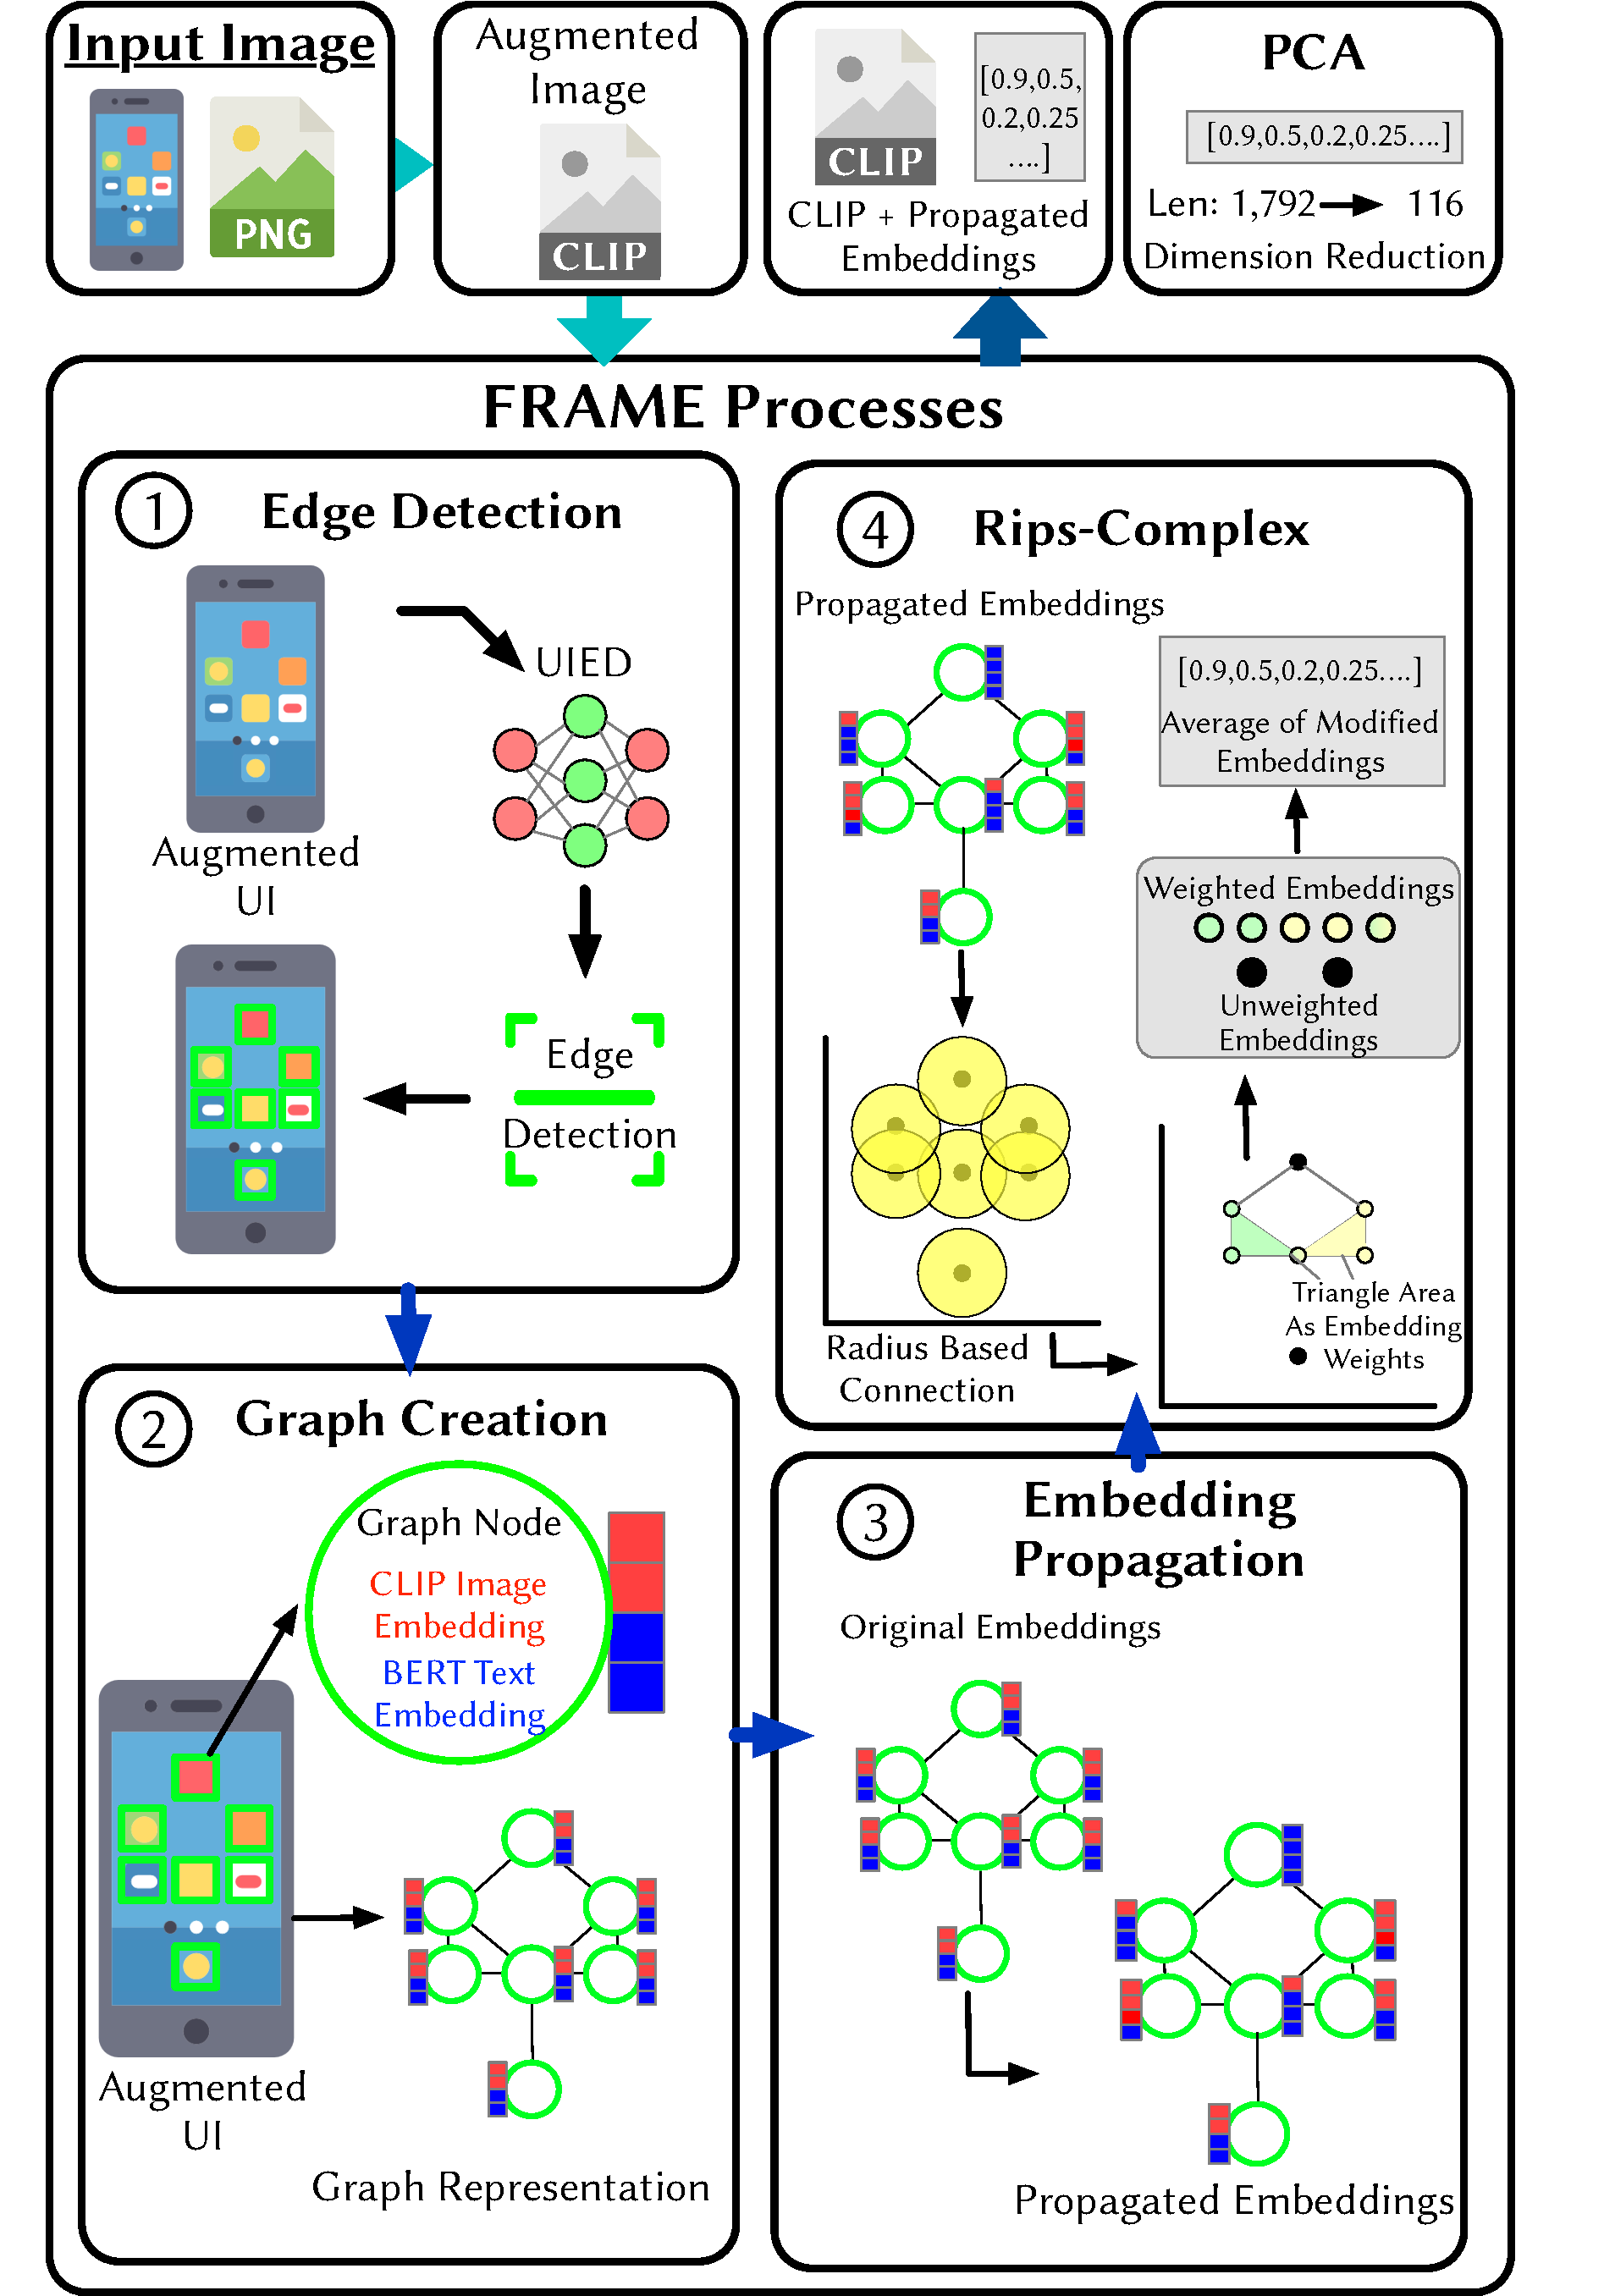
\includegraphics[width=0.6\textwidth]{imgs/FrameOverview.pdf}
    \caption{Overview of The FRAME Approach}
    \label{Overview}
\end{figure}

\FRAME is a structural-based approach to creating an image embedding that will aid in various screen similarity and retrieval tasks. To achieve this, \FRAME requires only the screenshot of a mobile app screen to generate the embedding. This is done as a way to maximize the use cases for \FRAME in any process that may require the embedding of a UI screen. \FRAME operates in five main stages to create the most structurally accurate representation of the screen. When a screen is given to \FRAME, it preprocesses the image using a series of image alteration techniques. We use the images and use edge detection to extract visual elements of the screen while retaining their positional information within the context of the screen. We create a graph-based representation of these elements and contextually weight the graph nodes based on their neighborhoods. Once that is done, \FRAME will take the new node embeddings and consolidate them using the Vietoris-Rips complex to consolidate the graph information into one embedding. The process of creating this embedding is visualized in Figure~\ref{Overview}. This embedding will be a structurally rich embedding which may aid in tasks requiring a numerical UI screen representation. 

\subsubsection{Pre Processing the Image}
Screens are designed to be visually pleasing and provide an intuitive placement of the elements such as icons and text boxes. In order for the embedding to abstract the elements on the screen and mitigate noise on the screen, \FRAME utilizes two screen preprocessing techniques. Noise on the screen can take many forms such as color palettes, customized icon designs, and different fonts. To mitigate these types of noise on the screen, \FRAME uses black-and-white as well as high contrast alterations to the screen. 
\subsubsubsec{black-and-white Modification}

\begin{figure}[h]
    \centering
    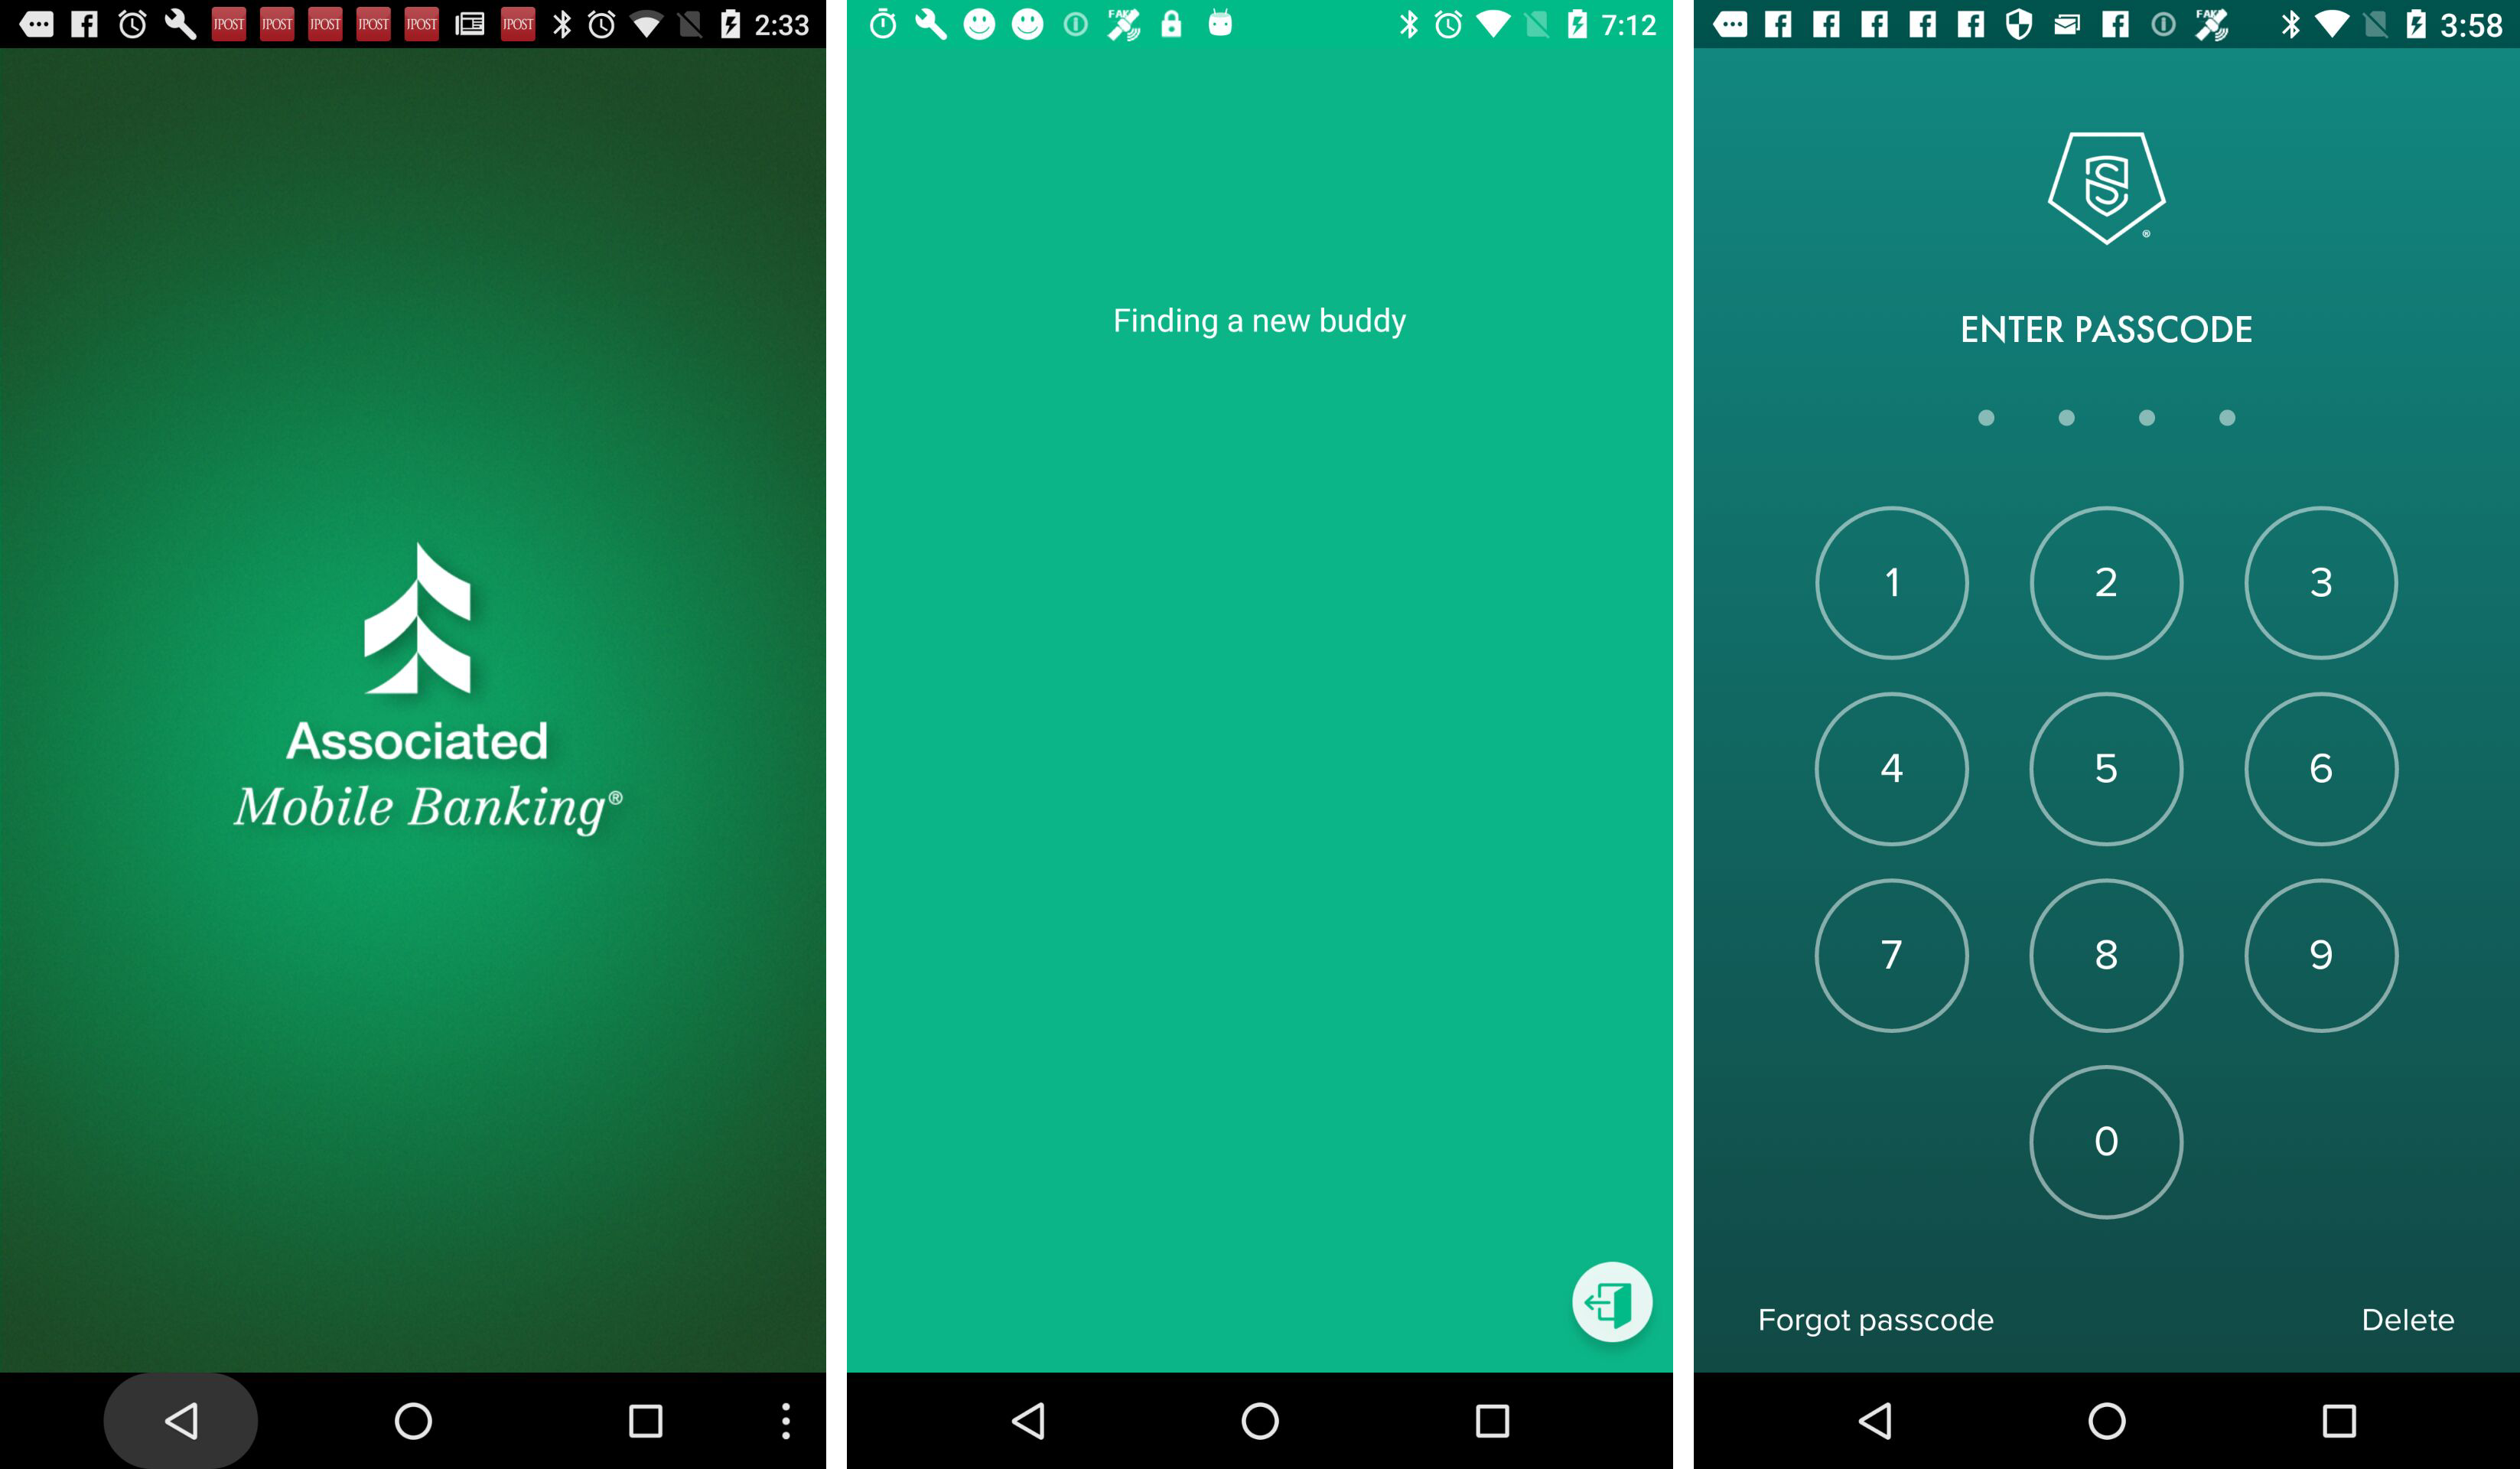
\includegraphics[width=0.55\textwidth]{imgs/3Clip.png}
    \caption{3 Similar Images using CLIP Embeddings}
    \label{3clip}
\end{figure}

\FRAME's goal is to provide skeletal-based similarity of screens rather than color. For example, Figure~\Ref{3clip} shows three images that were the most similar when using a CLIP embedding~\cite{clip}. The three screenshots have very similar color palettes and dominating colors upon visual inspection. On top of being similarly colored, these images do not share the same structural components and are three different types of screens. The leftmost screen is a Splash screen, the middle is a Search screen, and the rightmost screen is a password screen. Visual intuition suggests that these three screens provide different functions, but the CLIP embedding, which considers the colors of the screen, is unable to properly identify this discrepancy in the visual structure of the elements on the screen. To diminish the identified issues experienced by CLIP, we opt to remove color as a factor from consideration. We use the Pillow library's~\cite {pillow} grey scale conversion to convert the image to black-and-white first to ensure that no color is present in the extraction of the screen elements in the process of making the embedding. This can be seen in Figure~\ref{preprocessing} as the input image is made black-and-white. 


\begin{figure}[h]
    \centering
    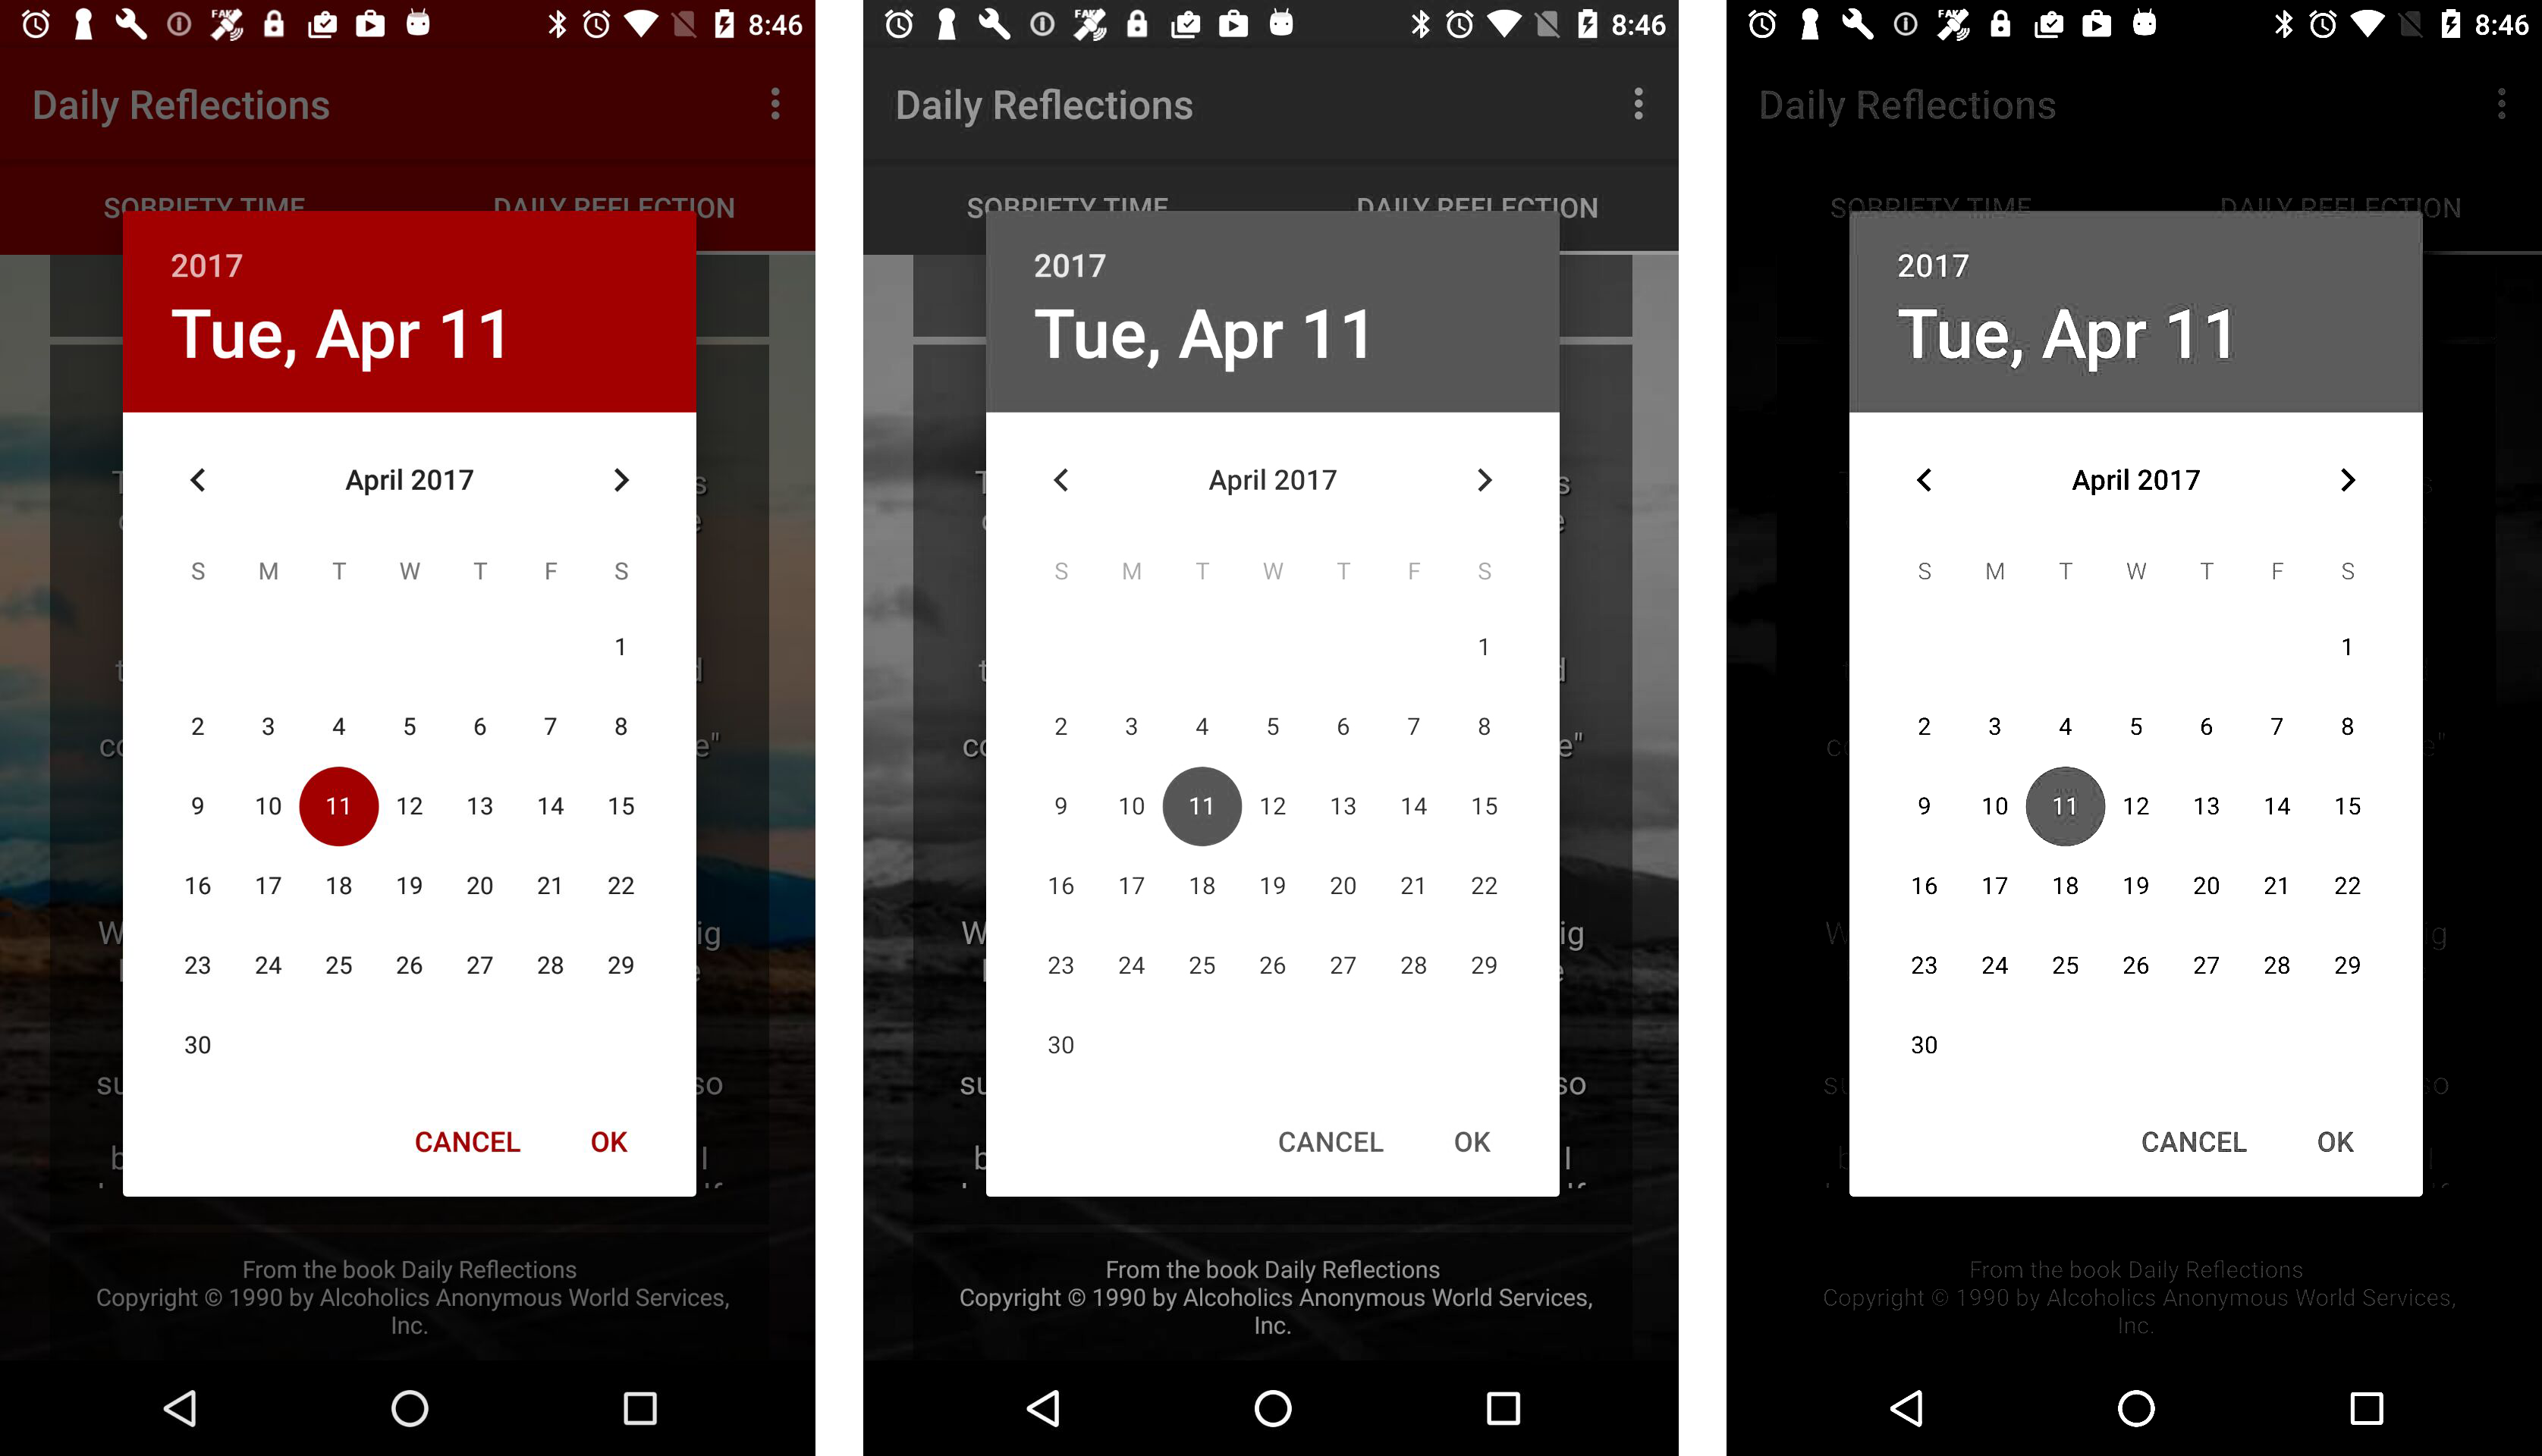
\includegraphics[width=0.55\textwidth]{imgs/PreProcessing.png}
    \caption{Preprocessing and augmenting the input image}
    \label{preprocessing}
\end{figure}

\subsubsubsec{High-Contrast} 


In addition to making each input screenshot black-and-white, we alter the images by increasing the contrast by 2X in the image. Contrast allows \FRAME to darken the dark pixels in the screen and brighten the brighter pixels in the screen. The resulting image has two main characteristics: (i) enhanced edge visibility; (ii) reduced noise influence. Enhanced edges are created because the colors on either side of the edge are modified, resulting in a more obvious and harsh edge. This aids the edge detection algorithm in finding accurate edges to accurately represent the screen's elements. Reduced noise is achieved by merging shades that are very close to each other, such as drop shadows, to create an abstract screen without many distractions for the edge detection algorithm. We use the Pillow library's~\cite{pillow} "ImageEnhance" sublibrary which has a contrast function to increase the contrast in the image. An example of this is shown in Figure~\ref{preprocessing}. We can see that the initial black-and-white image has less pronounced shades of greyscale colors and edges, while the high-contrast image has very clear boundaries between light and dark which can help facilitate edge detection. 


\subsubsection{Graph Creation}

To ingrain the visual structure of a UI screen, \FRAME utilizes a graph to plot nodes in similar areas as they appear on the screen. These nodes are created by the individual elements of the screen and their positional information. This positional information combined with elemental embedding information provides for a rich node within the graph to define relations between elements within the graph neighborhoods. There are three stages to developing a graph for each screen. 


\subsubsubsec{Edge Detection}

 \FRAME's goal is to create an embedding with the same intuitive structural pattern humans notice in their UIs. This is motivated by the examples of screens shown in Figure ~\ref{3clip}. We identify that passcode screens traditionally have the keypad in the center and that splash screens traditionally have the logo of the app in the center while surrounded by color. Being able to extract the icons and elements of the screen that suggest these patterns is a key element in creating an embedding that is capable of identifying these patterns. The edge detection approach used is an open-source edge detection model called UIED ~\cite{UIED}. UIED is specialized to work with UI Screens and provides high-quality element detection. This approach is further aided by the preprocessed image. \FRAME takes the edge detector's output and crops out each image. \FRAME only considers images larger than 48x48px since that is the standard for minimum accessible icons on an Android screen as per Google's Accessibility Guidelines ~\cite{GoogleAccess}. UIED gives the bounding box for each element as well, which can be used to find the centralized (x,y) point where the element is located on the screen. This is the positional information for each extracted element on the screen. 

\subsubsubsec{Graph Creation}


Icons on the screen have contextual information to offer to a screen. For example, a magnifying glass icon can indicate search, or a gear wheel icon may suggest settings. In addition to the positional information obtained through UIED, \FRAME takes into account the visual and textual aspects of each icon on the screen. To do this, we take the cropped icon provided by UIED and create 2 embeddings from it, an image embedding using CLIP, and a text embedding using BERT~\cite{BERT}.

\begin{figure}[h]
    \centering
    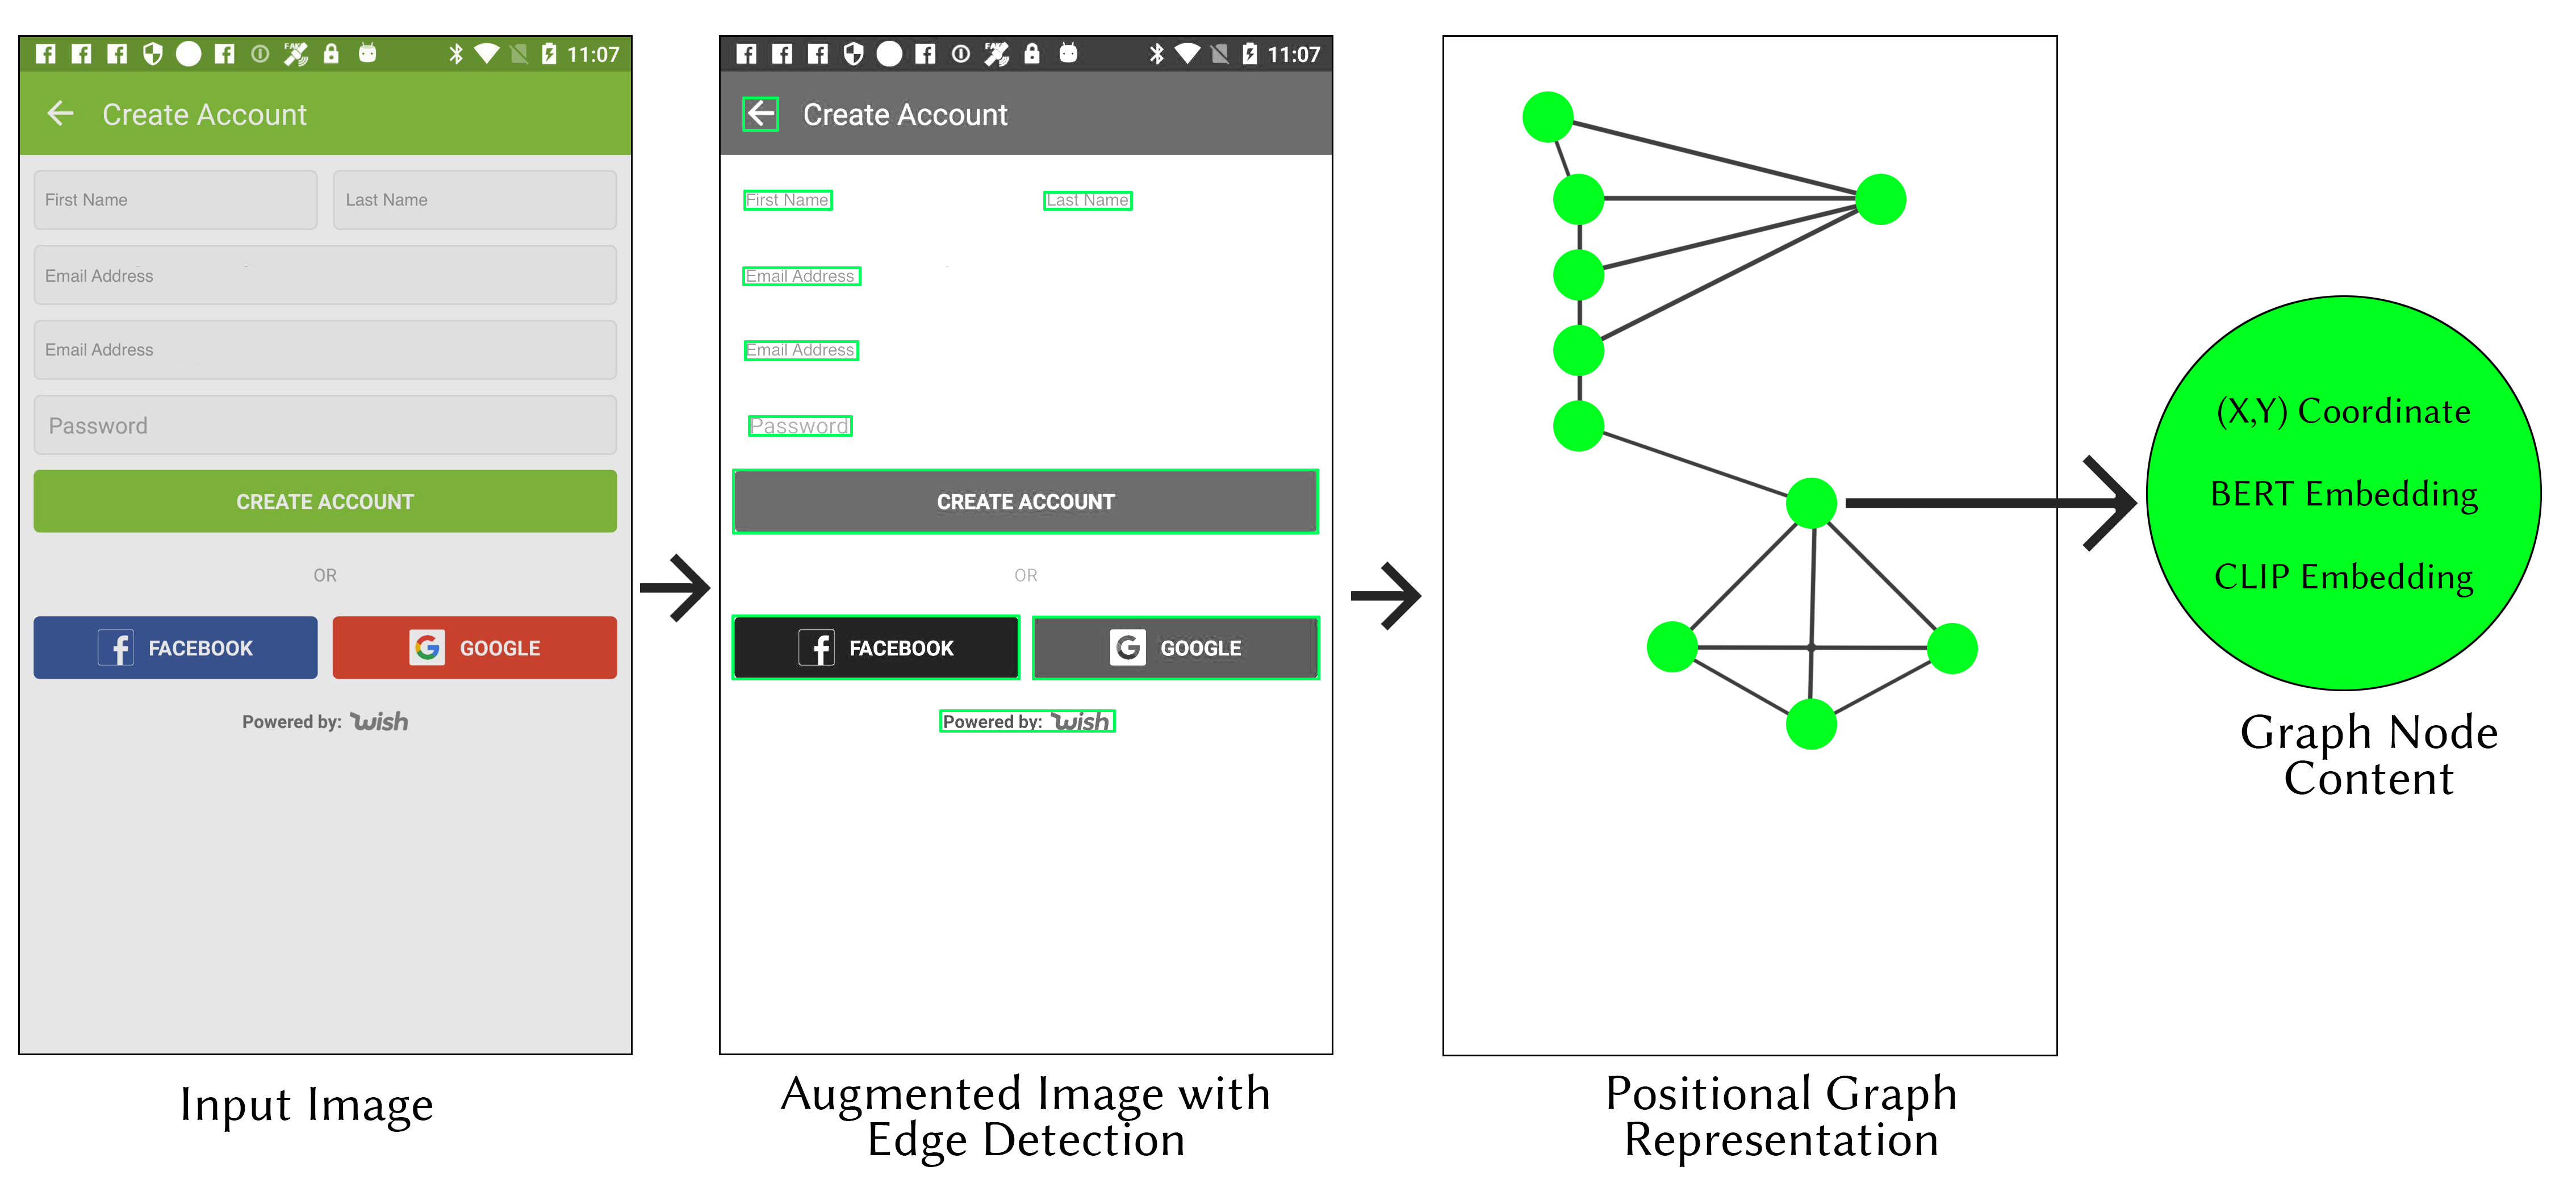
\includegraphics[width=0.7\textwidth]{imgs/graphCreation.png}
    \caption{Process of creating the graph}
    \label{graphCreation}
\end{figure}


\underline{\textit{Image Embedding:}} Though CLIP may not capture structure that well, CLIP is excellent at identifying stylistically similar screens as shown in Figure~\ref{3clip}. We use this property of CLIP to create embeddings for each icon on the screen. We create the icon embedding and add it to the node in the graph that represents the element on the screen. As shown in Figure~\ref{graphCreation}, each node has a visual representation of the icon that is cropped out of the screen.
 
\underline{\textit{Text Embedding:}} BERT is currently the most advanced text embedding available and we utilized it to create textual embeddings for each icon. Icons may have text in them, for example, the Facebook icon has the letter "F" and the word "Facebook" under the logo. We can leverage this text to add more depth to each node within the graph. We use PyTesseract to extract text from each cropped icon. We take the extracted text and clean it using regex functions to make it clean text. \FRAME takes the extracted, cleaned text and creates the BERT embedding to add to the graph node. As shown in Figure~\ref{graphCreation}, each node has a textual representation of the icon that is cropped out of the screen. In the case there is no text, a single space character is used as default. 

With the inclusion of the image and text embeddings within each node as well as the (x,y) positional coordinate for each icon, the nodes in the graph are filled with niche data that is localized to each icon. This gives each node a unique set of features that sets it apart from other nodes within the graph and its neighborhoods. We can utilize this diversity of node information to create a graph that can map relations between nodes based on their embedding data. 

\underline{\textit{Graph Edges:}} Once nodes for the graph are created, \FRAME takes into account the positional distance between the nodes in the graph and connects nodes that are within a certain distance to each other on the screen. The graph connects nodes that are a maximum of 300 pixels in distance from each other when using Manhattan distance. On average, the distance between icons on the screens is 300 pixels as observed by the authors. Therefore, we elected to use the average distance as the threshold for edge connection to ensure that the resulting graph does not lack edges or appear overly complete. This approach allows for the formation of distinct neighborhood clusters within the graph. The graph is built with nodes that have position coordinates, BERT embedding, and CLIP embedding and are connected via edges to form neighborhoods. This is shown in Figure~\ref{graphCreation}. \FRAME aims to find patterns between close elements, so having the connections be a maximum distance of 300 pixels allowed the graph to have distinct neighborhoods of nodes on different parts of the screen. This helps localize icon clusters and elements on the screen that may closely be related to each other. 



\subsubsection{Graph Embedding Propagation}
Unlike ordinary images, GUI screens exhibit a more structural nature, with closer relationships existing between adjacent components. Therefore, we augment the image/text embedding of each component by its neighbor component embeddings based on the constructed structural graph. This is inspired by a recent work for code embedding augmentation by leveraging the program dependence (i.e. structural) graph constructed for a software system  \cite{yanfu2024athena}. Specifically, our embedding propagation strategy is derived from the first-order approximation of localized spectral filters on graphs \cite{kipf2016semi, defferrard2016convolutional}, which can be represented as follows: 

\begin{equation} 
    S' = (I_N + w D ^ {-\frac{1}{2}} A  D ^ {-\frac{1}{2}}) S. 
\end{equation} 

$S \in \mathbb{R}^{N \times M}$ represents the matrix of all the image/text embeddings of nodes from $G$ and $S'$ represents the updated matrix by incorporating the information from the neighbor nodes. $M$ denotes the dimension of each image/text embedding (i.e. $768$) and $N$ denotes the number of nodes in the graph. $A$ is the adjacency matrix of $G$ without self-connections and $D$ is the degree matrix of $A$ so that the adjacency matrix is normalized by $D$ with respect to both the row and the column. $w$ is a constant to balance the information from the original node/component with structural information from the neighbor nodes/components. By leveraging the embedding propagation strategy, the image/text embedding for each component will encompass more structural information from its adjacent components, which is expected to further enhance GUI screen understanding. A visual representation of this process is shown in Figure \ref{Overview}-3.  


\subsubsection{Rips-Complex}

We realize the propagated UI embeddings as a set of points in Euclidean space to capture information regarding the topological relationship of the embedded data. This is achieved by triangulating the points to create a structure known as a simplicial complex as shown in Figure~\ref{fig:simplex}. 

\begin{figure}[h]
    \centering
    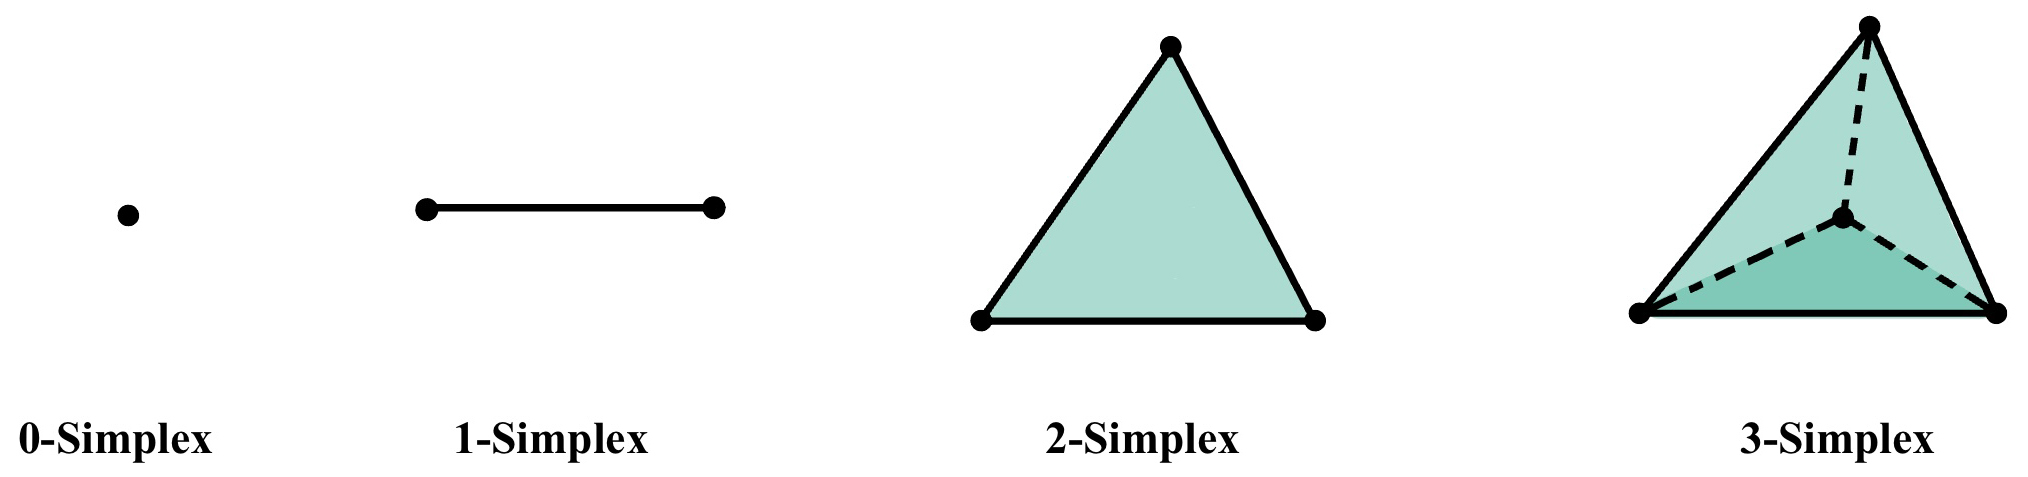
\includegraphics[width=0.6\textwidth]{imgs/simplexMod.jpg}
    \caption{Visualization of low dimensional simplicies}
    \label{fig:simplex}
\end{figure}

A simplicial complex is created by plotting the propagated embeddings on a graph in Euclidian space. We use our embeddings to create an object known as the Vietoris-Rips complex (often called the Rips complex) using GUHDI \cite{gudhi:RipsComplex}. Given a parameter $\epsilon>0$, the Rips complex of embeddings $\mathcal{X}$ is made into a simplicial complex that captures the spatial and topological relationships between the points in space using the following definition: 

\begin{definition}
Given a set of embeddings $\mathcal{X} = \{x_1, x_2, \hdots, x_k\} \subset \mathbb{R}^{n}$ and an $\epsilon>0$, a $k$-simplex $\sigma = [x_{i_1}, x_{i_2}, \hdots x_{i_k}]$ is in the Vietoris-Rips Complex $\textit{Rips}_{\epsilon}(\mathcal{X})$ if and only if:
\[ \mathbb{B}_{\epsilon}(x_{i_j}) \cap \mathbb{B}_{\epsilon}(x_{i_{j'}}) \neq \emptyset \]
where $\mathbb{B}_{\epsilon}(x_{i_j})$ is an open ball at $x_{i_j}$.
\end{definition}

\begin{figure}[h]
    \centering
    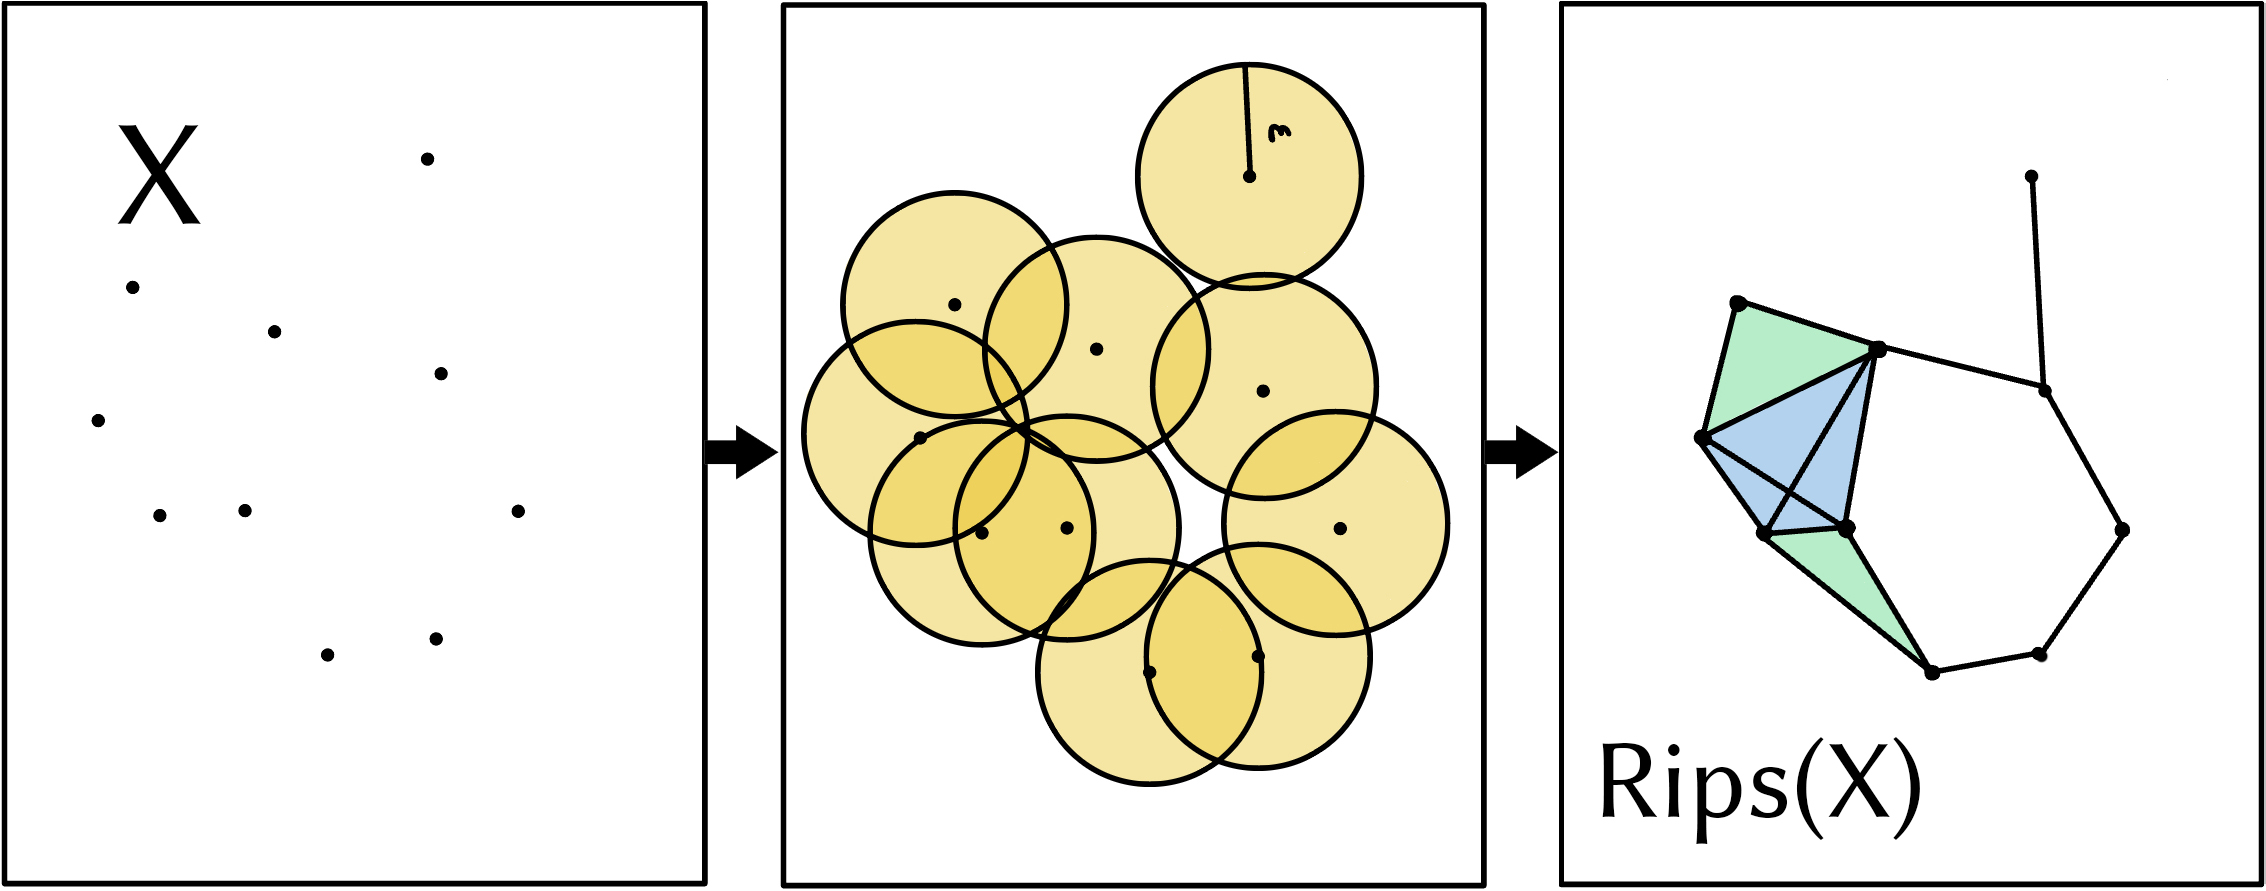
\includegraphics[width=0.6\textwidth]{imgs/RipsMod.jpg}
    \caption{Process of creating the Rips Complex using a set of embeddings}
    \label{fig:Rips}
\end{figure}

$\epsilon>0$ is the radius of the open ball used to determine edge connections within the embedding space. For small parameters of $\epsilon$, the open balls are too small to intersect and result in a complex with only the original embeddings. On the opposite end, if $\epsilon$ is too large, every feature in the input image is related to every other feature. We selected $\epsilon$ by performing a parameter study from $0.1-1$ in increments of $0.05$. Our ideal value of $\epsilon$ captures the average 100-200 features present in an input image. This was chosen to be $\epsilon=0.5$, as it resulted in an average of 100-200 $2$-simplicies generated in the Rips complex. The process of overlapping open balls and simplex creation is shown in Figure \ref{fig:Rips}. 

By employing the Rips complex on the propagated UI embeddings we are topologically capturing the relationship between an object in an image with all other objects in the image as shown in Figure \ref{fig:Rips}. Once the simplex is created, we consider the embeddings that make $2$-simplicies (2D triangles) and use the area of the resulting simplex as a weight for the involved embeddings. The area of a given 2-simplex can be calculated using Heron's formula \cite{weisstein2003heron}:
\begin{equation}
    \text{Area} = \sqrt{S(S-A)(S-B)(S-C)}
\end{equation}
\noindent where $S$ is the semi-perimeter of the 2-simplex and $A,B,$ and $C$ are the lengths of its three edges. The area is then used to weigh the involved embeddings.

We employ the Area-based Triangulated Embedding method (ATE), proposed by Krishna Vajjala et al. \cite{vajjala2024vietoris}, for the weighted average of the embeddings. This creates a weighted relation between embeddings that are close to each other, resulting in a weighted preservation of information between those three embeddings. We do this until we have a set of weighted and unweighted embeddings. We then average these embeddings together into one final embedding. A visual representation of this process is shown in Figure \ref{Overview}-4. 

\subsubsection{Final Embedding}

\FRAME embeddings reinforce existing embeddings by adding structural understanding to an image. The process of creating a distance-similar graph, propagating the embeddings within it, and consolidating them using the area-based triangulation creates a structure-encoded set of embeddings. This set of embeddings can then be added to the initial pre-processed CLIP image embedding. This results in an embedding that has the pre-processed version of the CLIP embedding along with the propagates structural relations between the icons on the screen which are a CLIP and BERT embedding combined. The resulting embedding is noisy and large with a size of 1,792 dimensions. To combat this, \FRAME uses PCA \cite{PCA}, a dimension reduction technique to reduce noise in high-dimension vectors. PCA takes a list of vectors and identifies the directions (principal components) where the data varies the most. By projecting the original data onto these principal components, PCA effectively reduces the dimensionality of the dataset while preserving as much of the original information as possible through linear transformations. We use Google's Scikit-Learn's~\cite{sklearn} PCA which takes as input a series of vectors and the desired size of the vector. We considered the training data vectors from both of our datasets and ran a hyperparameter study to determine the best size for the resulting vector. The resulting vector size is reduced from 1,792 down to 116. To ensure that new embeddings result in size 116 without re-running PCA on the dataset, we use PCA's transformation matrix and do a dot product with the initial noisy vector and the transformation matrix to obtain the 116 size representation of the new embedding. 

\subsection{Evaluation Methodology}

\setlist[questions,1]{label=RQ\arabic*.,ref=RQ\arabic*}
\setlist[questions,2]{label=(\alph*),ref=\thequestionsi(\alph*)}
In this section, we describe the procedure we used to evaluate \FRAME. To achieve our study goals, we formulated the following
four research questions:

\begin{itemize}
	\item{\textbf{RQ$_1$} \textit{How does \FRAME perform against other baselines in screen retrieval tasks}}
	\item{\textbf{RQ$_2$} \textit{How does \FRAME perform on various types screens against the best baseline?}}
        \item{\textbf{RQ$_3$} \textit{How important is the structural embedding propagation between graphs in order enhance the embedding ?}}
        \item{\textbf{RQ$_4$} \textit{How well does \FRAME leverage its ability to abstract the screen and disregard styling?}}
        
\end{itemize}

\subsubsection{{\FRAME Evaluation Database}}
\FRAME is designed to understand structural aspects of the screen. Screen retrieval tasks are a suitable benchmark for \FRAME since the embedding will need to effectively identify other screens with similar visual layouts regardless of colors and text differences. This means that the evaluation for \FRAME has to focus on screen similarity and retrieval tasks that require \FRAME to find screens labeled of the same category. 

We evaluate \FRAME with two different databases, Avgust~\cite{Avgust} and Aurora~\cite{khan24}. 

\subsubsubsec{Aurora Dataset} 
While creating the Aurora tool~\cite{khan24}, authors created a labeled version of the RICO dataset with a small subset of the images. The RICO dataset is a set of 66,000 unique UI screenshots~\cite{Rico}. However, this dataset is just a set of screens and they are not labeled. The labeled Aurora dataset was made by selecting a 1\% subset of RICO UI images randomly. Then they performed an unlabeled clustering of the images based on their visual properties. They used k-means clustering and clustered them into groups. The authors manually examined the clusters and collectively agreed to label them into 21 distinct categories. This process resulted in a high-quality dataset to evaluate screen retrieval and search algorithms. This dataset has 21 distinct categories and 1370 screens. It is a sparse dataset and can test \FRAME's ability to find similar screens in a dataset with lots of variability. We divide this dataset using a 90 to 10 train-test split for testing. The resulting evaluation dataset is 1233 train images and 137 test images. 

\subsubsubsec{Avgust Dataset}
The Avgust dataset is another subset of the RICO dataset. This dataset is obtained from the Avgust paper by Zhao et al.~\cite{Zhao:FSE22}. It has 25 labels with 2475 total screens. This dataset was manually labeled by 4 authors who mutually agreed on each screen's category. This is a dense daset with above 130 screens per category on average. For testing, we divide this dataset using a 90 to 10 train-test split. The resulting evaluation dataset is 2219 train images and 256 test images. 


\subsubsection{\textbf{RQ$_1$} \textit{How does \FRAME perform against other baselines in screen retrieval tasks?}}
\label{sec:eval_metrics}
To evaluate \FRAME, we use two common information retrieval metrics to test its ability to find similar screens properly; we use Hits@k and Mean Reciprocal Rank (MRR). 

\subsubsubsec{Hits@k}

Hits@K is a metric that evaluates the effectiveness of information retrieval systems by measuring how many relevant items appear within the top K results. It assesses the tool's ability to provide relevant content within a specified top K number of ranked items. For example, Hits@10 would quantify the percentage of relevant items found within the top 10 results. This metric is beneficial for evaluating search algorithms and retrieval tasks, as it prioritizes the most relevant results users will likely encounter. 

\begin{equation}
\text{Hits@}k = \frac{\text{Number of relevant items in top }k\text{ results}}{k}
\end{equation}

We perform Hits@k with three different K values, 1, 5, and 10. When using Hits@K, a higher K value can make for a more lenient evaluation, having smaller numbers results in a rigid evaluation of the embedding that can provide true insight into its performance. In our assessment of \FRAME, we input a test image labeled with a specific category, then examine the top K images most similar to the test image to determine how many of them share the same label. This gives us an accurate representation of how \FRAME is able to find similarly structured screens. We perform this evaluation on both the Aurora and the Avgust datasets to test its ability to find similar screens in sparse and dense datasets. 

\subsubsubsec{Mean Reciprocal Rank (MRR)}

Mean Reciprocal Rank (MRR) is a metric commonly used in information retrieval and ranking tasks. It calculates the average of the reciprocals of the ranks at which the relevant items are retrieved. For instance, if a relevant item is found at rank 3, its reciprocal would be \( \frac{1}{3} \). If another relevant item is found at rank 5, its reciprocal would be \( \frac{1}{5} \). The MRR is then calculated as the average of these reciprocals. 

\begin{equation}
\text{MRR} = \frac{1}{N} \sum_{i=1}^{N} \frac{1}{rank_i}
\end{equation}

MRR provides a single numerical value that summarizes the performance of the system across multiple queries, making it useful for evaluating and comparing different ranking algorithms or search models. In our assessment of \FRAME, we input a test image labeled with a specific category, then examine the list of images most similar to the test image to find the first image with the same label as the test image. This evaluation provides insight into how well \FRAME identifies similar images as higher in the list of similar images. We perform this evaluation on both the Aurora and the Avgust datasets to test its ability to find similar screens in sparse and dense datasets. 

It is important to understand how well \FRAME performs on its own, but having it perform the same tasks as other, common, baselines provides an insight into how well \FRAME is able to perform in information retrieval tasks. We take the same test and train data from both of our datasets and perform the same, rigorous, evaluation on three baselines to measure \FRAME's performance in comparison to the baselines. We compare \FRAME to three key baselines: CLIP, Screen2Vec, and BERT. We use these baselines to measure \FRAME 's efficacy compared to popular tools. 

\subsubsubsec{CLIP}

OpenAI's CLIP embeddings~\cite{clip} are currently the most popular embedding for image-related tasks. CLIP embeddings are capable of creating an embedding for any image regardless of it being a screen or not. However, CLIP has emerged as the prominent embedding given that they can represent both images and text in a shared embedding space, enabling cross-modal understanding. \FRAME takes into account the visual and textual aspects of the screen as well, so having CLIP embeddings given their popularity and their construction is a valuable baseline to \FRAME. 

\subsubsubsec{Screen2Vec}


Li et al.'s Screen2Vec ~\cite{Li21} is designed as an embedding specifically for screens. This serves as a valuable baseline in evaluating the performance of \FRAME because Screen2Vec is designed to embed UI screens and so is \FRAME. This baseline allows us to test \FRAME against another screen-specific embedding.  

\subsubsubsec{BERT}

Google's BERT embeddings ~\cite{BERT} serve as a good baseline for \FRAME because it is a widely-used and well-understood model for natural language understanding tasks. Despite being primarily designed for text processing, BERT can still encode textual information about images, providing a simple and readily available baseline for cross-modal tasks. 

We use these three baselines and the same information retrieval metrics presented above to evaluate \FRAME 's performance in comparison to the baselines. 

\subsubsection{\textbf{RQ$_2$} \textit{How does \FRAME perform on various types of screens against the best baseline?}}

To determine \FRAME's ability to detect various screens, we present a case study aimed at evaluating the performance of \FRAME across various types of screens, comparing its performance against the best baseline. The study focuses on different screen functionalities such as login, search, etc., to provide a comprehensive understanding of \FRAME's efficacy in diverse contexts. 

To conduct the case study, we identify the best baseline against which to compare \FRAME's performance. This baseline is chosen based on the most similar performance to \FRAME when considering the metrics presented in Section \ref{sec:eval_metrics}, considering its robustness and reliability in similar contexts. Additionally, we implemented both \FRAME and the best baseline in the same test and train splits across both Avgust and Aurora datasets to ensure there is a thorough, fair comparison.

\subsubsection{\textbf{RQ$_3$} \textit{How important is the structural embedding propagation between graphs in order enhance the embedding ?}}

Embedding propagation is the process of modifying embeddings within a neighborhood to weigh nodes differently. This process aids in weighting embeddings based on their structural proximity. This process provides the structural-based enhancement to the base CLIP embedding. To determine \FRAME's ability to structurally enhance the base embedding, it is important to consider \FRAME's performance with and without its embedding propagation. There are six variants of embedding propagation that we test against the final variant of \FRAME. In the interest of space and simplicity, we have elected to create codes for each variant of \FRAME. The structure is as follows: C-PB-PC. This indicates the augmented CLIP, the propagated BERT, and the propagated CLIP embeddings are all present within the variant. To omit an embedding to create a variant, we add an \textbf{'N'} next to the embedding. For example: NC-PB-PC indicates that the augmented CLIP embedding is \textbf{not} present, but the propagated BERT and CLIP embeddings are present. Below are the descriptions of each variant along with their codes for reference. 

\subsubsubsec{Propagated Embedding: NC-PB-PC}

The propagated embedding has both the CLIP and BERT propagated embeddings that are concatenated with the original modified CLIP embedding. This set of concatenated propagated embeddings provides the foundation to enhance the modified CLIP embedding with structural properties. To demonstrate the need for propagated embedding in the final embedding, we run the same set of tests that the \FRAME embedding is evaluated with, but we omit the augmented CLIP embedding and only leave the propagated embedding. In return, this will demonstrate the performance impact that the CLIP has within the \FRAME embedding.

\subsubsubsec{CLIP + No Propagated CLIP: C-PB-NPC}

The propagated embedding has both the CLIP and BERT propagated embeddings that are concatenated with the original modified CLIP embedding. The propagated CLIP embedding is a weighted CLIP embedding that is created by the propagation between graph nodes within a neighborhood. This relationship is crucial to adding image-based structural properties to the image since the approach weighs images that are closer to each other.  To demonstrate the need for propagated CLIP embeddings in the final embedding, we run the same set of tests that the \FRAME embedding is evaluated with, but we omit the propagated CLIP embedding and leave in propagated BERT embedding and augmented CLIP embedding. In return, this will demonstrate the performance impact that CLIP embedding propagation has within the \FRAME embedding. 

\subsubsubsec{CLIP + No Propagated BERT: C-NPB-PC}

The propagated embedding has both the CLIP and BERT propagated embeddings that are concatenated with the original modified CLIP embedding. The propagated BERT embedding is a weighted BERT embedding that is created by the propagation between graph nodes within a neighborhood. This relationship is crucial to adding textual-based structural properties to the image since the approach weighs text within icons that are closer to each other.  To demonstrate the need for propagated BERT embeddings in the final embedding, we run the same set of tests that the \FRAME embedding is evaluated with, but we omit the propagated BERT embedding and leave in propagated CLIP embedding and augmented CLIP embedding. In return, this will demonstrate the performance impact that BERT embedding propagation has within the \FRAME embedding. 

\subsubsubsec{CLIP + No Propagated Embeddings: C-NPB-NPC}

The propagated embedding has both the CLIP and BERT propagated embeddings that are concatenated with the original modified CLIP embedding. This set of concatenated propagated embeddings provides the foundation to enhance the modified CLIP embedding with structural properties. To demonstrate the need for propagated embedding in the final embedding, we run the same set of tests that the \FRAME embedding is evaluated with, but we omit the propagated embeddings and only leave the augmented CLIP embedding. In return, this will demonstrate the performance impact that the propagated embedding has within the \FRAME embedding.

\subsubsubsec{Only Propagated BERT: NC-PB-NPC}

Propagated embeddings carry intrinsic spatial data with weights depending on their proximity to other elements on the screen. However, it is important to consider the performance of the propagation itself. We do this by running the same tests that the \FRAME embedding is evaluated with, but only consider the propagated BERT embedding. 

\subsubsubsec{Only Propagated CLIP: NC-NPB-PC}

Propagated embeddings carry intrinsic spatial data with weights depending on their proximity to other elements on the screen. However, it is important to consider the performance of the propagation itself. We do this by running the same tests that the \FRAME embedding is evaluated with, but only consider the propagated CLIP embedding. 

\subsubsection{\textbf{RQ$_4$} \textit{How well does \FRAME leverage its ability to abstract the screen and disregard styling?}}

To determine \FRAME's ability to disregard stylistic elements in a UI, it is important to consider \FRAME's performance with and without its various screen augmentations. \FRAME performs a black-and-white augmentation first and then adds on a high contrast augmentation to remove color bias in the screen and create more defined objects on the screen. To test the efficacy of these techniques, we run an augmentation study to determine how much each augmentation impacts the resulting performance for \FRAME. We do this by testing three different variants of \FRAME. In the interest of space and simplicity, we have elected to create codes for each variant of \FRAME in the augmentation study. The structure is as follows: B-C. This indicates the augmented input image has both black-and-white and contrast augmentations. To omit an augmentation to create a variant, we add an \textbf{'N'} next to the augmentation. For example: B-NC indicates that the augmented input image has a black-and-white augmentation but the high contrast augmentation is \textbf{not} present. Below are the descriptions of each variant along with their codes for reference.

\subsubsubsec{No Contrast: B-NC}

\FRAME uses contrast enhancement to aid the computer vision in identifying elements on the screen. This is necessary to avoid extracting elements that could be slight color variations or small on the screen. This gives \FRAME the highest quality elements to use in its graph and reduces the number of unrelated elements in the propagation. To demonstrate the need for contrast enhancements in the image, we run the same set of tests that the \FRAME embedding is evaluated with, but we omit the contrast augmentation and leave in the other augmentations to the embedding including the embedding propagation and the black-and-white augmentation. In return, this will demonstrate the performance impact that contrast provides within the \FRAME embedding. 

\subsubsubsec{No black-and-white: NB-C}
\FRAME converts the input image to black-a
nd-white to remove a color bias in the similarity measure. This is important since it eliminates the ability for the embedding to make similar embeddings solely off color and allows \FRAME to enhance the embedding with structural properties. To demonstrate the need for black-and-white enhancements to the image, we run the same set of tests that the \FRAME embedding is evaluated with, but we omit the black-and-white conversion and leave in the other augmentations to the embedding including the embedding propagation and the contrast enhancements. In return, this will demonstrate the performance impact that black-and-white provides within the \FRAME embedding. Thus proving the motivation that color-independent screen similarity tasks are structurally influenced.

\subsubsubsec{No Contrast and No black-and-white: NB-NC}

To demonstrate the need for augmentation, it is important to consider the performance of the embedding without any augmentation. \FRAME embeddings are motivated by the idea that the embedding should have no color and style bias, unlike popular image embeddings. To do this, we built \FRAME to remove colors from the image being processed. This intuition serves well for the idea behind \FRAME, but it is important to show that this intuition results in higher performance. %\FRAME increases the contrast in the image to create harsher edges to aid the computer vision model in finding elements on the screen. These two techniques combined serve as the base for the larger embedding.
To demonstrate that these augmentations are necessary, we run the same set of tests that the \FRAME embedding is evaluated with, but we omit all initial enhancements while retaining the embedding propagation. In return, this will demonstrate the performance impact that the preprocessing steps provide within the \FRAME embedding. Thus strengthening the motivation behind the augmentation decisions.


\subsection{Evaluation Results}

This section analyzes the results of our empirical evaluation of \FRAME. 

\subsubsection{\textbf{RQ$_1$} \textit{How does \FRAME perform against other baselines in screen retrieval tasks?}}

\begin{table}[h]
\centering
\renewcommand{\arraystretch}{1} % Adjust the row height
\scalebox{1}{
\begin{tabular}{|c|c|c|c|c|c|}
\toprule
\textbf{Dataset} & \textbf{Metrics} & \textbf{Screen2Vec} & \textbf{BERT} & \textbf{CLIP} & \textbf{FRAME} \\
\hline
\midrule
\multirow{4}{*}{Aurora} & HR@1 & 0.3750 & 0.3194 & 0.4722 & \textbf{0.5625*} \\
& HR@5 & 0.3027 & 0.2486 & 0.4013 & \textbf{0.4652*} \\
& HR@10 & 0.2604 & 0.2187 & 0.3590 & \textbf{0.4166*} \\
& MRR & 0.4853 & 0.4363 & 0.5963 & \textbf{0.6729*} \\
\hline
\hline
\multirow{4}{*}{Avgust} & HR@1 & 0.3922 & 0.8270 & 0.8549 & \textbf{0.8784*} \\
& HR@5 & 0.3185 & 0.7788 & 0.7788 & \textbf{0.8266*} \\
& HR@10 & 0.2739 & 0.7141 & 0.7364 & \textbf{0.7799*} \\
& MRR & 0.5116 & 0.8908 & 0.8913 &  \textbf{0.9138*} \\
\bottomrule
\end{tabular}
}
\caption{Results over 2 datasets, where the best results are in \textbf{bold}, and \textbf{*} indicates a p-value less than 0.05 from two-tailed paired t-test between FRAME and best baseline (CLIP). }
\label{MainResults}
\end{table}

\noindent \FRAME performs significantly better in screen retrieval tasks compared to the state-of-the-art baseline methods. Specifically, \FRAME outperforms Screen2Vec, BERT, and CLIP in every metric for both datasets. It is important to note that Screen2Vec is designed as an embedding for UI screens, BERT is used in image embeddings by extracting the text on the screen to identify semantic similarities between screens, and CLIP is the leading image embedding method that leverages textual and visual properties of images. From the results in Table \ref{MainResults}, we can see that, compared to the best baseline, \FRAME shows an average of 15.9\% improvement on the Aurora dataset and an average of 4.3\% improvement on the Avgust dataset. The Aurora dataset contains fewer images and is more sparse overall, making the screen retrieval task difficult. On the other hand, the Avgust dataset is very dense and contains a large number of screens. Given that the two datasets are very different in nature, \FRAME is able to show superior performance in screen retrieval tasks across both datasets along with statistically significant results. In addition, for the Aurora dataset, the MRR improvement between \FRAME and the best baseline is roughly 12.8\% and the improvement between \FRAME and the best baseline for the Avgust dataset is 2.5\%. The MRR metric gives higher scores to screens that appear closer to the top of a ranked list. Based on these results, we show \FRAME's impressive ability to rank similar UI screens towards the top of the ranked list.



\begin{table}[h]
\centering
\renewcommand{\arraystretch}{1} % Adjust the row height
\scalebox{0.75}{
\begin{tabular}{|c|c|c|c|c|c|c|c|c|c|c|}
\toprule
\textbf{Dataset} & \textbf{Metrics} & \textbf{NC-NPB-PC} & \textbf{NC-PB-NPC} & \textbf{C-NPB-NPC} & \textbf{NC-PB-PC} & \textbf{C-PB-NPC} & \textbf{C-NPB-PC} & \textbf{FRAME}\\
\hline
\midrule
\multirow{4}{*}{Aurora} 
& HR@1 & 0.2777 & 0.3750 & 0.4722 & 0.4166 & 0.5138 & 0.4513 & \textbf{0.5625}\\
& HR@5 & 0.1944 & 0.2972 & 0.4013 & 0.2750 & 0.4486 & 0.4180 & \textbf{0.4652}\\
& HR@10 & 0.1631 & 0.2791 & 0.3590 & 0.2458 & \textbf{0.4180} & 0.3618 & 0.4166\\
& MRR & 0.3880 & 0.5026 & 0.5963 & 0.5136 & 0.6448 & 0.6077 &\textbf{0.6729} \\
\hline
\hline
\multirow{4}{*}{Avgust} 
& HR@1 & 0.7960 &  0.8352 & 0.8549 & 0.8666 & 0.8588 & 0.8705 & \textbf{0.8823}\\
& HR@5 & 0.6901 &  0.7850 & 0.7788 & 0.8023 & 0.8282 &  0.8219 & \textbf{0.8329}\\
& HR@10 & 0.5929 & 0.7360 &  0.7364 & 0.7498 & 0.7721 & 0.7674 & \textbf{0.7827} \\
& MRR & 0.8380 &  0.8724 & 0.8913 & 0.9012 & 0.9014 & 0.9114 & \textbf{0.9184}\\
\bottomrule
\end{tabular}
}
\caption{Ablation analysis over 2 datasets between \FRAME and its variants, where the best results are in \textbf{bold}.}
\label{AblatioTable}
\end{table}

\subsubsection{\textbf{RQ$_2$} \textit{How does \FRAME perform on various types of screens against the best baseline?}}

It is important to evaluate \FRAME on fine grained datapoints in addition to the averaged metrics. We evaluated \FRAME and its best baseline, CLIP, to gain a finer understanding of their performance on various screen types. We present a head-to-head comparison against the two embeddings using Hits@10. Hits@10 strikes a balance between precision (the proportion of relevant results among the retrieved items) and recall (the proportion of relevant results that are successfully retrieved). By considering only the top 10 results, Hits@10 emphasizes precision while still providing a reasonable measure of recall, giving a holistic view of each embedding's capabilities. 

\begin{figure}[h]
    \centering
    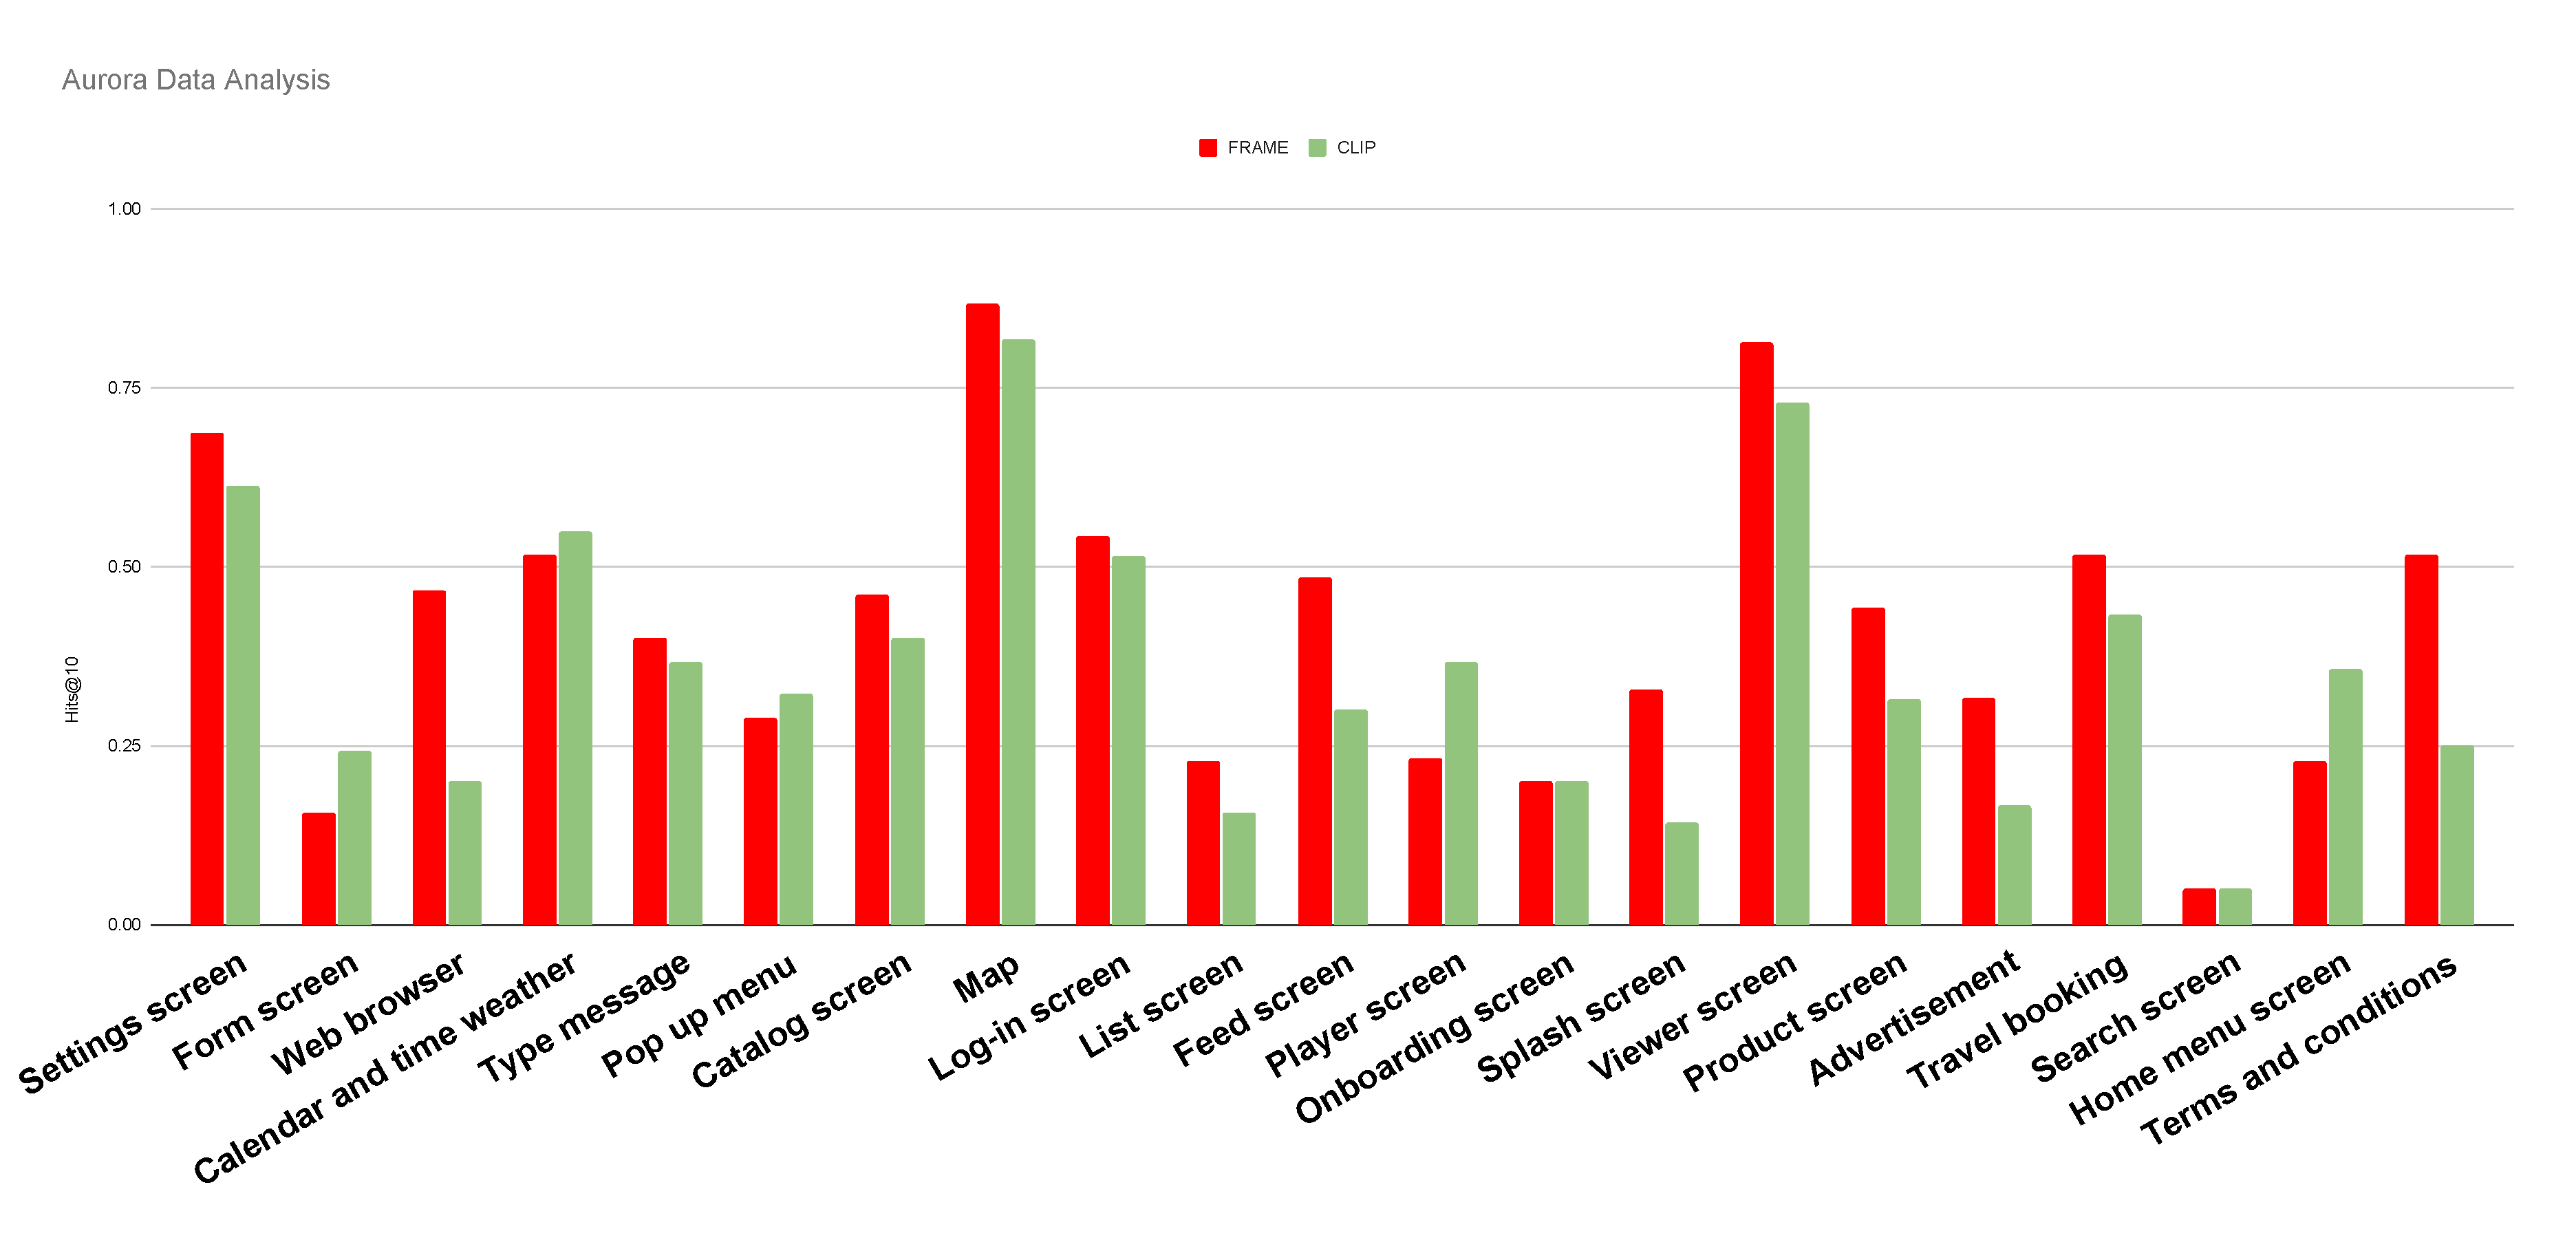
\includegraphics[width=0.75\textwidth]{imgs/AuroraCase.pdf}
    \caption{Visualization of FRAME vs CLIP Hits@10 on different screen types in the Aurora dataset}
    \label{fig:AuroraCase}
\end{figure}

Figure \ref{fig:AuroraCase} presents the difference between FRAME and CLIP embeddings on various screen types in the Aurora dataset. The bar chart shows \FRAME in red and CLIP in green. We see that \FRAME outperforms CLIP in every category except for four screen types. This gives \FRAME an advantage above CLIP in 17/21 screen categories. In the context of UI screen retrieval, the \FRAME embedding's advantage over CLIP embedding's performance across 17 out of 21 screen categories highlights \FRAME 's efficacy in capturing nuanced visual features specific to UI elements. \FRAME's performance in comparison to CLIP suggests that Frame embeddings are better suited for tasks requiring precise understanding and representation of static UI screens, potentially leading to improved retrieval accuracy and user experience in UI-related applications. 

\begin{figure}[h]
    \centering
    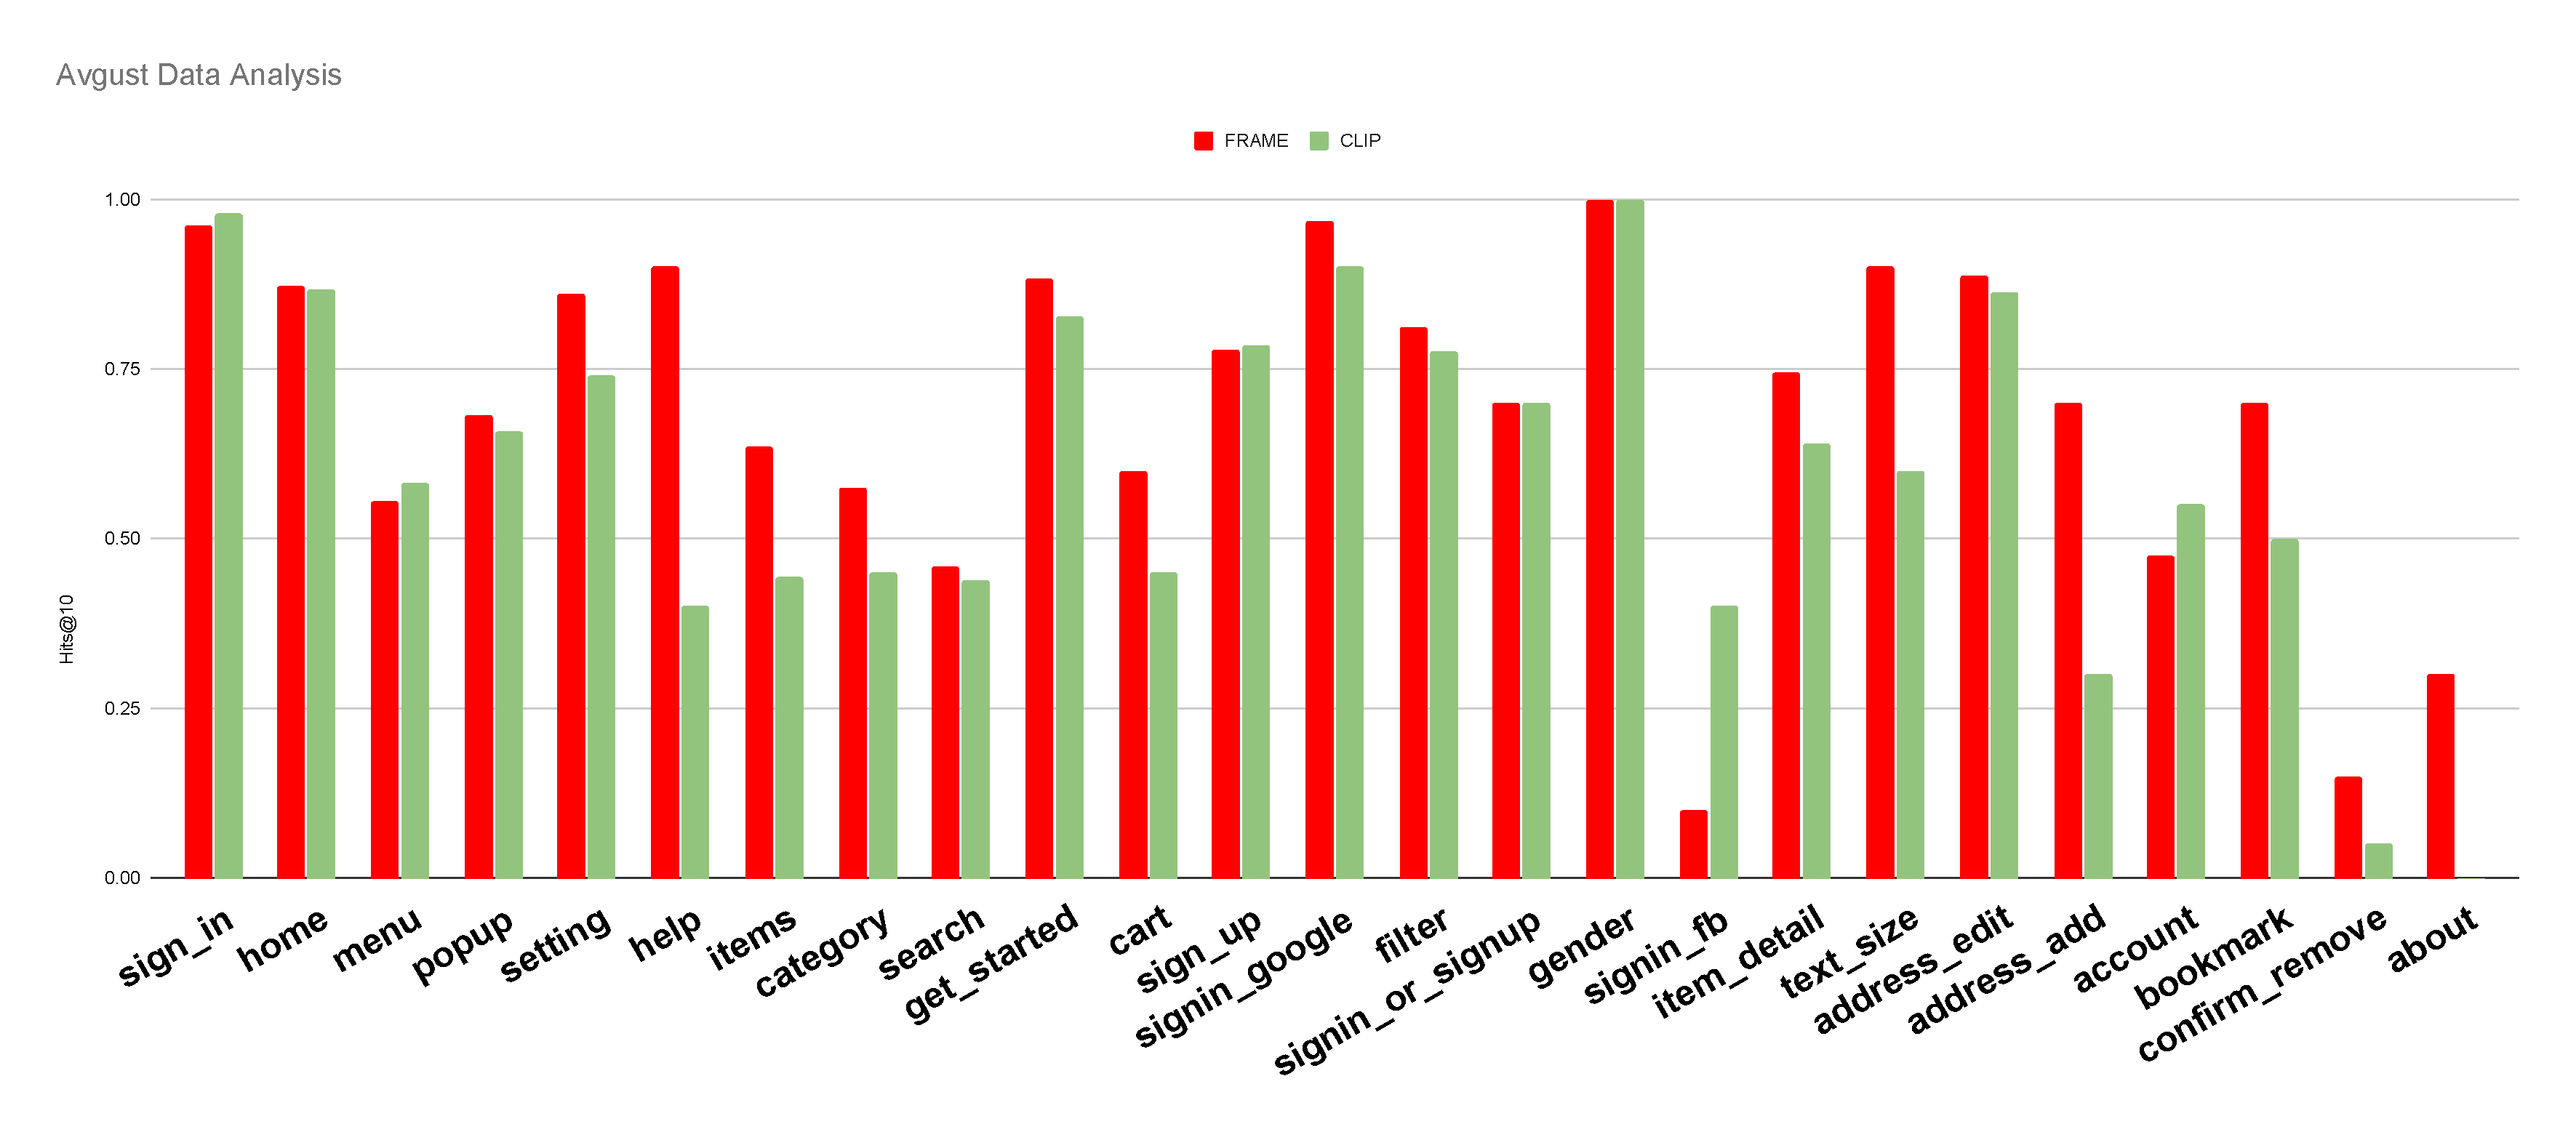
\includegraphics[width=0.75\textwidth]{imgs/AvgustCase.pdf}
    \caption{Visualization of FRAME vs CLIP Hits@10 on different screen types in the Avgust dataset}
    \label{fig:AvgustCase}    
\end{figure}

Figure \ref{fig:AuroraCase} presents the difference between FRAME and CLIP embeddings on various screen types in the Avgust dataset. The bar chart shows \FRAME in red and CLIP in green. We see that \FRAME outperforms CLIP in every category except for four screen types. This gives \FRAME an advantage above CLIP in 20/25 screen categories. In the context of UI screen retrieval, the \FRAME embedding's advantage over CLIP embedding's performance across 20 out of 25 screen categories highlights \FRAME 's efficacy in capturing nuanced visual features specific to UI elements. \FRAME's performance in comparison to CLIP suggests that Frame embeddings are better suited for tasks requiring precise understanding and representation of static UI screens, potentially leading to improved retrieval accuracy and user experience in UI-related applications. 


\subsubsection{\textbf{RQ$_3$} \textit{How important is the structural embedding propagation between graphs in order to enhance the embedding?}}


\FRAME creates a graph representation of the screen and augments weights within the nodes based on proximity and neighborhoods. This approach is designed to provide a set of weighted embeddings that can ingrain structural information into the embedding. To demonstrate the need for this propagation, we conduct an ablation study with six different variants of \FRAME, including and excluding various properties from the embedding. Table~\ref{AblatioTable} has the results for the ablation study for both datasets with each variant of \FRAME. \FRAME outperforms all variants of frame in every metric except for the version of frame that has the modified CLIP embedding and the propagated CLIP embedding in Hits@10 on the Aurora dataset. As described in Section ~\ref{sec:eval}, there are 6 variants of \FRAME. Table~\ref{AblatioTable} shows a comparison of \FRAME's results to all the variants.  
In the variants that do not have the larger augmented CLIP embedding and have one of the two possible propagated embeddings, Variants: NC-NPB-PC and NC-PB-NPC, we see poor performance. This poor performance can be attributed to the lack of broader screen information. These variants are solely dependent on the propagation between the icons or the text on the screen. 

In the variants that do have the larger augmented CLIP embedding and have one of the two possible propagated embeddings, Variants: C-NPB-PC and C-PB-NPC, we see an improved performance to the previous two variants. However, these variants still underperform when compared to the results for \FRAME. Given the lower performance of these two variants, it is assumed that the presence of both propagated is important to provide a higher structural context for the overall embedding. 

Given the results of the other four embeddings, \FRAME has two more configurations which offer a direct insight into the impact of the modified CLIP embedding and propagated embedding inclusion. 
The two main configurations to consider are NC-PB-PC and C-NPB-NPC. 

\begin{itemize}
  \item \textbf{NC-PB-PC}: This variant of \FRAME only has the propagated CLIP and BERT embedding. This is the information that ingrains the modified CLIP with structural information. However, on its own, the propagated embeddings are the fourth best variant of \FRAME. It outperforms the augmented version of CLIP which is just an image with no structural enhancements. This is shown in Table~\ref{AblatioTable}.
  \item \textbf{C-NPB-NPC}: This variant of \FRAME only has the augmented CLIP embedding without the propagated CLIP and BERT embeddings. This is the base image that is going to be enhanced with structural context. This variant of \FRAME is only the third best variant of \FRAME, only beating out the individual propagated CLIP and BERT embeddings, as shown in Table~\ref{AblatioTable}.
\end{itemize}

However, together, \FRAME can combine the two variants and leverage the properties of the augmented CLIP embedding and the structural properties of the propagated embeddings to create a structure-biased embedding. This results in \FRAME outperforming every variant of itself, demonstrating the impact of each element within the ablation process. 

\subsubsection{\textbf{RQ$_4$} \textit{How well does \FRAME leverage its ability to abstract the screen and disregard styling?}}
\begin{table}[h]
\centering
\renewcommand{\arraystretch}{1} % Adjust the row height
\scalebox{1}{
\begin{tabular}{|c|c|c|c|c|c|}
\toprule
\textbf{Dataset} & \textbf{Metrics} & \textbf{NB-C} & \textbf{NB-NC} & \textbf{B-NC} & \textbf{FRAME} \\
\hline
\midrule
\multirow{4}{*}{Aurora} 
& HR@1 & 0.4930 & 0.5347 & 0.5208 & \textbf{0.5625} \\
& HR@5 & 0.4069 & 0.4250 & 0.4527 & \textbf{0.4652} \\
& HR@10 & 0.3638 & 0.3805 & 0.4138 & \textbf{0.4166} \\
& MRR & 0.6171 & 0.6484 & 0.6492 & \textbf{0.6729} \\
\hline
\hline
\multirow{4}{*}{Avgust} 
& HR@1 & 0.8505 & 0.8784 & 0.8784 & \textbf{0.8823} \\
& HR@5 & 0.8119 & 0.8298 & 0.8266 & \textbf{0.8329} \\
& HR@10 & 0.7658 & 0.7827 & 0.7799 & \textbf{0.7827} \\
& MRR & 0.9094 & 0.9118 &  0.9138 &  \textbf{0.9184} \\
\bottomrule
\end{tabular}
}
\caption{Results over 2 datasets, where the best results are in \textbf{bold}, between FRAME and its variants including both contrast and black and white. }
\label{AugmentationTable}
\end{table}

\FRAME addresses color and style bias limitations in prior work by augmenting the image. There are three image preprocessing variants for the \FRAME embedding. The results for this augmentation ablation study are presented in Table~\ref{AugmentationTable}.

\subsubsubsec{NB-C}
This variant of \FRAME only increases the contrast on the input image. The results show that increasing the contrast on the input image is the least effective form of augmentation. As shown in Table~\ref{AblatioTable}, this variant of \FRAME is the least effective. 

\subsubsubsec{B-NC} 
This variant of \FRAME does not increase the contrast in the input image and only converts it to greyscale. The results show a noticeable increase in the performance of this variant, making it the highest-performing variant behind \FRAME. This variant benefits from the lack of color and allows the embedding to take on the structural aspects of the propagated embedding without allowing color bias to play a factor. 

\subsubsubsec{NB-NC}
This variant of \FRAME does not increase the contrast or make the image black-and-white. The results for this variant are interesting since it outperformed the contrast only variant. This gives an insight into how important the black-and-white is for the high contrast augmentation to define clear edges. 

Together with the inclusion of the black-and-white and high contrast modification, \FRAME can create an embedding that outperforms its variants while excluding color and increasing edge detection capabilities to define elements clearly on the screen. 


\FRAME is a novel approach to enhance existing image embeddings with structural information to embed UIs. There has been limited work in this area, so we present related work that has similar concepts to what \FRAME tries to achieve. We looked at previous work in UI Embeddings, UI Search and similarity, and Graph Based UI Representations. 

\subsection{Embedding Related Works}
There exists a limited body of work when considering embeddings for UI screens~\cite{Li21}, however, there have been increased efforts to provide a screen-specific embedding. 

One such effort is Screen2Vec, proposed by Li et al.~\cite{Li21}. Screen2Vec tackles the lack of UI Screen embeddings and proposes its own neural embeddings. Screen2Vec uses BERT text embeddings to take into account the text on the screen. Additionally, they use a layout embedding to embed the images with some layout information. Screen2Vec differs by creating their own embedding while using the Rico data~\cite{Rico} and uses the extracted screen hierarchy to embed screen hierarchy. This layout-based screen embedding is also employed by Deka et al. in Rico~\cite{Rico}. Both of these approaches use the same layout-based screen embedding which differs from the \FRAME proposes. These two embedding techniques aim to create a new embedding while \FRAME aims to enhance an existing embedding to be suitable for screen structure. 
\FRAME uses a computer vision approach to find the elements on the screen and use their positional information on the screen as opposed to finding elements within the screen hierarchy. \FRAME also utilizes a graph-based approach to creating layouts while considering both element visual and text characteristics within the graph. 

Li et al.~\cite{li2021vut} proposed VUT, a UI transformer for multimodal multi-task user interface modeling. This approach considered the hierarchical structure, image, and language properties of the screen to create their screen representations. VUT has two Transformer architectures, an Image-Structure model,
and a Question-Answer model. The image-structure model combines screenshot and view hierarchy data for UI encoding while the question-answer model encodes questions while attending to UI encodings from the Image-Structure model, generating text answers for language tasks and serving as the question encoder for grounding tasks to locate UI elements for action. However, \FRAME is a lightweight approach that takes existing embeddings and enhances them with structural properties and does not create its embedding using a transformer architecture. The structural properties of the screen in \FRAME are graph and visual position-based as opposed to hierarchy-based representation in VUT. VUT is an excellent baseline comparison for \FRAME, however, the model and architecture to use VUT are currently unavailable to the public. 

Bai et al.~\cite{bai2021uibert} proposed UIBert, a transformer-based joint image-text model to learn generic feature representations for a UI and its components~\cite{bai2021uibert}. This embedding is similar to VUT in its goal to create an embedding using image, text, and structural properties of the screen. Similar to VUT, UIBert also considers the view hierarchies for each screen and the leaf nodes. UIBert uses the element information on the screen in conjunction with the visual text to create an embedding with both textural and structural information. However, as discussed with VUT, UIBert is a new transformer-based embedding framework, whereas \FRAME enhances existing embeddings. Additionally, \FRAME interprets structure as visual positions on the GUI rather than an image's position in the hierarchy. UIBert may have provided an insight into the performance of \FRAME as a baseline, however, the models for UIBert are not available to the public. 

\subsubsubsec{UI Search and Similarity}
This paper presents a retrieval-motivated image embedding. It is important to consider other ways screen retrieval has been done ~\cite{Huang19, Bernal-Cardenas19, Chen20} and how \FRAME can be used to enhance search based on its retrieval-based evaluation. Guigleproposed by Bernal-Cardenas et al.~\cite{Bernal-Cardenas19} is a UI search engine. They use metadata information to facilitate a filter-based search. This method of finding embeddings is functional but does not provide and mbedding based search. Search is done through filters to find an image. 

GeminiScope proposed by Mao et al.~\cite{Mao18} proposed a GUI similarity metric that uses the leaf nodes in the hierarchy tree to determine the position of the elements on the screen. They compute the absolute values of UI-related features,
such as position and size, and use these metrics as their numerical representation for the screen. This allows them to perform distance calculations on the different images based on UI feature locations. \FRAME, like GeminiScope, considers the position of UI elements on the screen. However, GeminiScope does not consider the relations between the embeddings, unlike \FRAME. Additionally, \FRAME considers the text on the screen along with the actual visual representation of the icons. 

\subsubsubsec{UI Comprehension}
To modify or test a UI, it is necessary to have a semantic understanding of the UI. Many tools use the android screen hierarchy~\cite{bai2021uibert,li2021vut, Li21, Schoop22}, however, the hierarchy is not always available. We present a prior work that has used computer vision techniques to gain a semantic understanding of the elements on the screen. 
Spotlight, a tool introduced by Li et al.~\cite{li20spotlight} is a tool that uses computer vision to create a vision-language model architecture that can assist in screen comprehension tasks. Spotlight can generate text to suggest a screen or icon's function. This helps create lightweight icon detection for screens without a hierarchy. Following this line of thinking, we designed \FRAME to be hierarchy-free and use a computer vision approach to detect icons on the screen, resulting in an embedding that only needs a screenshot as input. 

Additionally, Schoop et al. ~\cite{Schoop22} proposed a technique to classify tappable icons on a screen given an image. This work is done by using XRAI. XRAI identifies and emphasizes influential areas within the input screenshot, which affect the prediction of capability for the chosen region. Additionally, it employs k-Nearest Neighbors to showcase mobile UIs from the dataset that exhibit contrasting influences on the perception of tappability. Though the intended application was not related to screen embedding creation, tappable icons can uncover important relations within the way the icons on a screen are laid out. \FRAME does not consider the tappability of the icon, however, it is a direction that can be considered. \FRAME is concerned with identifying niche relationships between icons and where they are positioned on the screen as opposed to their functionality. 

\subsubsubsec{Graph Based UI Representation}
Li et al. proposed Sugilite~\cite{Li20-suglite}, a graph-based UI element search for UI screens. Sugilite creates a UI snapshot graph using element metadata and position to identify each element on the screen. This allows users to write test scripts to test certain elements of the screen using natural language queries. WHile this is not an embedding, it utilizes a similar intuition to \FRAME by considering the graph-based approach to mapping elements. This method differs from \FRAME in two ways. Sugilite does not perform any structural relationship analysis between the different elements, they use the graph as a means to query the UI and find elements. Sugilite also uses metadata from the UI screens to create the graph. \FRAME aims be more versatile, therefore it creates an embedding for a screen from only the image of the screen. 

\subsection{Summary}
In this paper, we presented \FRAME, an approach for enhancing UI screen embeddings with structural information. We measured the performance and generalizability of \FRAME to various open source UIs. Our results indicate that \FRAME is effective in practice and outperforms key baselines, offering a novel approach to create vectors for UIs. Future work will examine the potential create embeddings for web apps and focus on creating an entirely new embedding as opposed to enhancing current ones.











